% This template is used for pandoc
\documentclass[10pt]{ctexart}

\def\university{Harbin Institute of Technology}
\def\team{Dolls in Pseudo Paradise}
\def\season{2024-2025}

\usepackage{amsmath, amssymb}
\usepackage{graphicx}
\usepackage{float}

% ==================== Begin     Page ====================
%%%%%% fix pandoc
\providecommand{\tightlist}{\setlength{\itemsep}{0pt}\setlength{\parskip}{0pt}}
\newcommand{\passthrough}[1]{#1}

\usepackage[a4paper, includehead, headsep=0.1in, left=0.4in, right=0.1in, top=0.1in, bottom=0.1in, landscape]{geometry}
\ctexset{
    section = {
        beforeskip = { 1.5ex plus 1ex minus .2ex },
        afterskip  = { 1.3ex plus .2ex }
    },
    subsection = {
        beforeskip = { 1.25ex plus 1ex minus .2ex },
        afterskip  = { 0.5ex plus .2ex }
    },
    subsubsection = {
        beforeskip = { 1.25ex plus 1ex minus .2ex },
        afterskip  = { 0.5ex plus .2ex }
    },
}

% Three columns & landscape to make the code tight
\usepackage{multicol}
\setlength{\columnsep}{30pt}

% ==================== Begin     Font ====================
\usepackage{fontspec}
\setmonofont{FiraCode-Regular.ttf}[
    Path = utils/,
    BoldFont = FiraCode-Bold.ttf,
    ItalicFont = FiraCode-Light.ttf,
    BoldItalicFont = FiraCode-Medium.ttf,
    Contextuals=Alternate           % Activate the calt feature
]

\setCJKmainfont{SourceHanSerif-Regular.otf}[
    Path = utils/,
    BoldFont = SourceHanSans-Regular.otf,
    ItalicFont = SourceHanSerif-Light.otf
]

\newCJKfontfamily[jinwen]\jinwen{DFJinwen-W3}[
    Path = utils/,
    Extension = .otf,
]

% ==================== Begin   Header ====================
\usepackage{fancyhdr}
\usepackage{zref-totpages}
\usepackage{epigraph}
\pagestyle{fancy}
\fancyhf{} % Clear up default styles

\setlength{\headheight}{12.08003pt}

% Header Left: University + team name
\fancyhead[L]{\university -- \textit{\team}}

% Header Center: Section
\fancyhead[C]{\leftmark}

% Header Right: Page number
\fancyhead[R]{Page \thepage\ of \ztotpages}

% Header line
\renewcommand{\headrulewidth}{0.4pt}

%%%%%% Main Content

\usepackage{xcolor}
\usepackage{listings, lstfiracode} % https://ctan.org/pkg/lstfiracode

% Color Palletes from Gihub
\lstset{
  language=[11]C++,
  basicstyle    = \ttfamily\small\color[HTML]{24292E},
  style=FiraCodeStyle,   % Use predefined FiraCodeStyle
  keywordstyle    =\color[HTML]{D73A49}\bfseries,
  commentstyle    =\color[HTML]{6A737D},
  numberstyle     =\color[HTML]{005CC5}\bfseries\sffamily,
  stringstyle     =\color[HTML]{032F62}\bfseries,
  tabsize = 2,
  breaklines,
  basewidth={0.6em, 0.5em},
  breakindent = 1.1em,
  columns = fixed,
  numbers = left,
  frame = single,
  lineskip=-1pt
}

% from https://github.com/4thcalabash/code_library/blob/master/tex/format.tex
% an amazing script
% converts an line-number to arbitrary string
\let\othelstnumber=\thelstnumber
\def\createlinenumber#1#2{
    \edef\thelstnumber{%
        \unexpanded{%
            \ifnum#1=\value{lstnumber}\relax
             \tt #2%
            \else}%
        \expandafter\unexpanded\expandafter{\thelstnumber\othelstnumber\fi}%
    }
    \ifx\othelstnumber=\relax\else
      \let\othelstnumber\relax
    \fi
}

% Only 1 and 2 level
\setcounter{tocdepth}{2}

\begin{document}

\begin{titlepage}
    \thispagestyle{empty}

    \vspace*{-1cm}

    \hfill
    \parbox{0.5\textwidth}{
        \epigraph{
            \textsf {Our village of honest men originally consisted of only eight people.} \\
            \textsf {We all picked up and moved to a mountain in the east. Two years of honest and boring daily life passed us by.} \\
            \textsf {One day, one of us found a little hole by a peach tree.} \\
            \textsf {Yes, after that we wandered into this paradise.} \\
            \textsf {And right away, I quit being human.}
        }{\textit{--- Dolls in Pseudo Paradise}}
    }
    \hspace{0.5cm}

    \vfill
    
    \begin{center}
        \Huge {\jinwen 蓬莱人形}算法模板库 \\
        \huge {\textsc{Reference Document} for \textsl{\team}}
    \end{center}

    \vspace*{2cm}

    \begin{figure}[htbp]
        \centering
        \begin{minipage}[c]{0.25\textwidth}
            \centering
            
\includegraphics[width=6cm]{utils/images/hit-logo.png}
        \end{minipage}
        \hspace{1cm}
        \begin{minipage}[c]{0.25\textwidth}
            \centering
            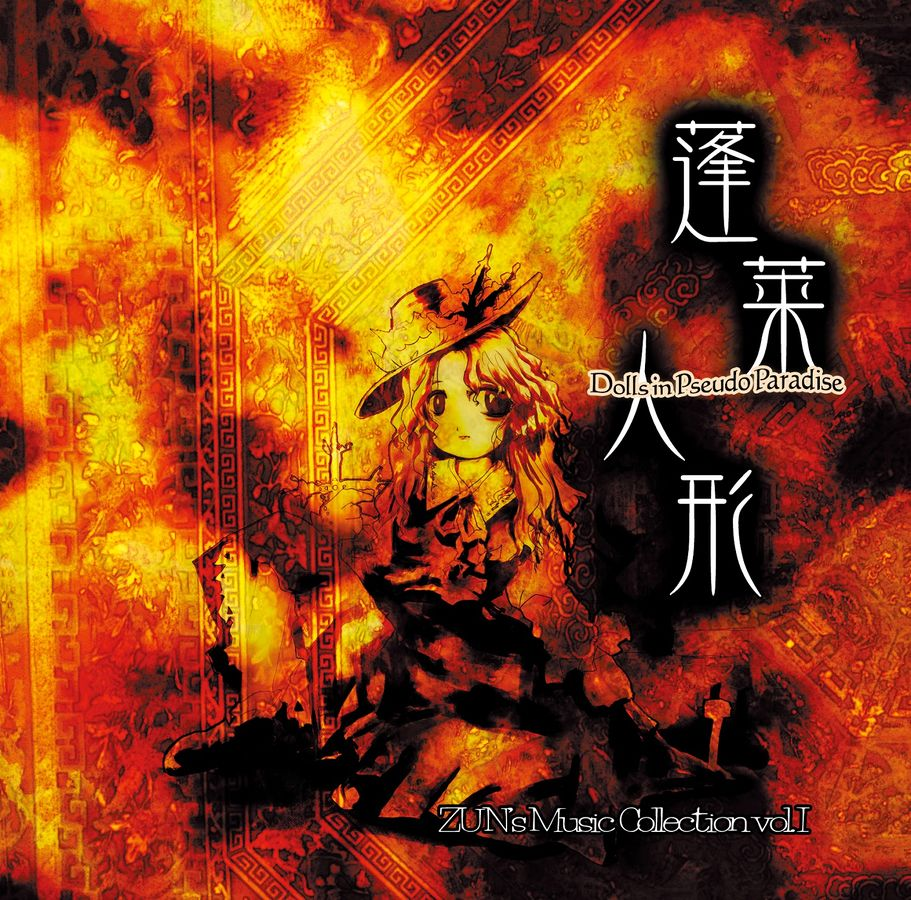
\includegraphics[width=6cm]{utils/images/hourai.jpg}
        \end{minipage}
        \hspace{1cm}
        \begin{minipage}[c]{0.25\textwidth}
            \centering
            
\includegraphics[width=6cm]{utils/images/icpc.png}
        \end{minipage}
    \end{figure}

    \vfill

    \begin{center}
        \Large \color{darkgray} \season \\
        \Large \color{darkgray} \university
    \end{center}

    \vspace*{1cm}
\end{titlepage}

\newpage

\begin{multicols}{3}
    \setcounter{page}{1}

    \tableofcontents
    
    \section{动态规划}\label{ux52a8ux6001ux89c4ux5212}

    \subsection{斜率优化}\label{ux659cux7387ux4f18ux5316}

    \subsubsection{形式}\label{ux5f62ux5f0f}

    考虑一个经典的 dp 转移方程如下:

    \[f_i = \max_{j < i}\{f(j) + w(j, i)\}\]

    我们将式子拆成三个部分:只跟 \(i\) 有关或者与 \(i,j\) 均不相关的部分
    \(a(i)\),只跟 \(j\) 有关的部分 \(b(j)\),跟 \(i,j\) 均有关的部分
    \(c(i,j)\):

    \[f_{i} = a(i) + \max_{j<i} \{b(j)+c(i,j)\}\]

    斜率优化可被用来解决这样一个情形:\(c(i,j)=ic_j\)。此时
    \(b(j)+c(i,j)\) 可视作关于 \(j\) 的一次函数。如果 \(c_j\) 随着 \(j\)
    的增大而单调,那么可用单调栈维护;否则可以考虑 CDQ
    分治或者在凸包上二分。在凸包上可以使用二分查询最高/最低点。

    \subsubsection{例题}\label{ux4f8bux9898}

    玩具装箱。原始转移方程为:

    \[f_i = \max_{j< i}\{f_j + (s_i-s_j-L')^2\}\]

    其中 \(s_i = i+\sum_{j\le i}c_i, L'=L+1\)。将其分类得到:

    \[
    \begin{aligned}
    f_i &= \max_{j<i}\{f_j+s_i^2+s_j^2+L'^2-2s_is_j+2s_jL'-2s_iL' \} \\
    &= (s_i^2 -2s_iL'+ L'^2) + \max_{j<i}\{(f_j+s_j^2+2s_jL') -2s_is_j \}
    \end{aligned}
    \]

    在原始的玩具装箱中,\(s_j\)
    单调增加,也就是斜率单调增加。因此可以直接使用单调栈维护凸包。同时
    \(s_i\) 也单调增加,因此可以用指针维护。

\begin{lstlisting}[language={C++}]
#include "../header.cpp"
int n, L, p, e, C[MAXN], Q[MAXN];
f80 S[MAXN], F[MAXN];
f80 gtx(int x){ return S[x]; }
f80 gty(int x){ return F[x] + S[x] * S[x]; }
f80 gtw(int x){ return -2.0 * (L - S[x]); }
f80 gtk(int x,int y){ return (gty(y) - gty(x)) / (gtx(y) - gtx(x)); }
int main(){ 
  cin >> n >> L;
  for(int i = 1;i <= n;++ i){
    cin >> C[i];
    S[i] = S[i - 1] + C[i];
  }
  for(int i = 1;i <= n;++ i){
    S[i] += i;
  }
  e = p = 1, L ++, Q[p] = 0;
  for(int i = 1;i <= n;++ i){
    while(e < p && gtk(Q[e], Q[e + 1]) < gtw(i))
      ++ e;
    int j = Q[e];
    F[i] = F[j] + pow(S[i] - S[j] - L, 2);
    while(1 < p && gtk(Q[p - 1], Q[p]) > gtk(Q[p], i))
      e -= (e == p), -- p;
    Q[++ p] = i;
  }
  printf("%.0Lf\n", F[n]);
  return 0;
}
\end{lstlisting}

    \section{数据结构}\label{ux6570ux636eux7ed3ux6784}

    \subsection{平衡树}\label{ux5e73ux8861ux6811}

    \subsubsection{无旋 Treap}\label{ux65e0ux65cb-treap}

\begin{lstlisting}[language={C++}]
#include "../../header.cpp"
mt19937_64 MT(114514);
namespace Treap{
  const int SIZ = 1e6 + 1e5 + 3;
  int F[SIZ], C[SIZ], S[SIZ], W[SIZ], X[SIZ][2], sz;
  u64 H[SIZ];
  int  newnode(int w){
    W[++ sz] = w, C[sz] = S[sz] = 1; H[sz] = MT();
    return sz;
  }
  void pushup(int x){
    S[x] = C[x] + S[X[x][0]] + S[X[x][1]];
  }
  pair<int, int> split(int u, int x){
    if(u == 0)
      return make_pair(0, 0);
    if(W[u] > x){
      auto [a, b] = split(X[u][0], x);
      X[u][0] = b, pushup(u);
      return make_pair(a, u);
    } else {
      auto [a, b] = split(X[u][1], x);
      X[u][1] = a, pushup(u);
      return make_pair(u, b);
    }
  }
  int merge(int a, int b){
    if(a == 0 || b == 0)
      return a | b;
    if(H[a] < H[b]){
      X[a][1] = merge(X[a][1], b), pushup(a);
      return a;
    } else {
      X[b][0] = merge(a, X[b][0]), pushup(b);
      return b;
    }
  }
  void insert(int &root, int w){
    auto [p, q] = split(root, w  );
    auto [a, b] = split(   p, w - 1);
    if(b != 0){
      ++ S[b], ++ C[b];
    } else b = newnode(w);
    p  = merge(a, b);
    root = merge(p, q);
  }
  void erase(int &root, int w){
    auto [p, q] = split(root, w  );
    auto [a, b] = split(   p, w - 1);
    -- C[b], -- S[b];
    p  = C[b] == 0 ? a : merge(a, b);
    root = merge(p, q);
  }
  int  find_rank(int &root, int w){
    int x = root, o = x, a = 0;
    for(;x;){
      if(w <  W[x])
        o = x, x = X[x][0];
      else {
        a += S[X[x][0]];
        if(w == W[x]){
          o = x; break;
        }
        a += C[x];
        o = x, x = X[x][1];
      }
    }
    return a + 1;
  }
  int  find_kth(int &root, int w){
    int x = root, o = x, a = 0;
    for(;x;){
      if(w <= S[X[x][0]])
        o = x, x = X[x][0];
      else {
        w -= S[X[x][0]];
        if(w <= C[x]){
          o = x; break;
        }
        w -= C[x];
        o = x, x = X[x][1];
      } 
    }
    return W[x];
  }
  int  find_pre(int &root, int w){
    return find_kth(root, find_rank(root, w) - 1);
  }
  int  find_suc(int &root, int w){
    return find_kth(root, find_rank(root, w + 1));
  }
}
\end{lstlisting}

    \subsection{珂朵莉树}\label{ux73c2ux6735ux8389ux6811}

\begin{lstlisting}[language={C++}]
#include "../header.cpp"
namespace ODT {
  // <pos_type, value_type>
  map <int, long long> M;
  // 分裂为 [1, p) 和 [p, +inf),返回后者迭代器
  auto split(int p) {
    auto it = prev(M.upper_bound(p));
    return M.insert(
      it,
      make_pair(p, it -> second)
    );
  }
  // 区间赋值
  void assign(int l, int r, int v) {
    auto it = split(l);
    split(r + 1);
    while (it -> first != r + 1) {
      it = M.erase(it);
    }
    M[l] = v;
  }
  // // 执行操作
  // void perform(int l, int r) {
  //   auto it = split(l);
  //   split(r + 1);
  //   while (it -> first != r + 1) {
  //     // Do something...
  //     it = next(it);
  //   }
  // }
};
\end{lstlisting}

    \subsection{可并堆}\label{ux53efux5e76ux5806}

\begin{lstlisting}[language={C++}]
#include "../header.cpp"
namespace LeftHeap{
  const int SIZ = 1e5 + 3;
  int W[SIZ], D[SIZ], L[SIZ], R[SIZ], F[SIZ], s;
  bool E[SIZ];
  int merge(int u, int v){
    if(u == 0 || v == 0)
      return u | v;
    if(W[u] > W[v] || (W[u] == W[v] && u > v))
      swap(u, v);
    int &lc = L[u];
    int &rc = R[u];
    rc = merge(rc, v);
    if(D[lc] < D[rc])
      swap(lc, rc);
    D[u] = min(D[lc], D[rc]) + 1;
    if(lc != 0) F[lc] = u;
    if(rc != 0) F[rc] = u;
    return u;
  }
  void pop(int &root){
    int root0 = merge(L[root], R[root]);
    F[root0] = root0;
    F[root ] = root0;
    E[root ] = true;
    root = root0;
  }
  int top(int &root){
    return W[root];
  }
  int getfa(int u){
    return u == F[u] ? u : F[u] = getfa(F[u]);
  }
  int newnode(int w){
    ++ s;
    W[s] = w;
    F[s] = s;
    D[s] = 1;
    return s;
  }
}
\end{lstlisting}

    \subsection{Link Cut 树}\label{link-cut-ux6811}

\begin{lstlisting}[language={C++}]
#include "../header.cpp"
namespace LinkCutTree{
  const int SIZ = 1e5 + 3;
  int F[SIZ], C[SIZ], S[SIZ], W[SIZ], A[SIZ], X[SIZ][2], size;
  bool T[SIZ];
  bool is_root(int x){ return X[F[x]][0] != x && X[F[x]][1] != x;}
  bool is_rson(int x){ return X[F[x]][1] == x;}
  int  new_node(int w){
    ++ size;
    W[size] = w, C[size] = S[size] = 1;
    A[size] = w, F[size] = 0;
    X[size][0] = X[size][1] = 0;
    return size;
  }
  void push_up(int x){
    S[x] = C[x] + S[X[x][0]] + S[X[x][1]];
    A[x] = W[x] ^ A[X[x][0]] ^ A[X[x][1]];
  }
  void push_down(int x){
    if(!T[x]) return;
    int lc = X[x][0], rc = X[x][1];
    if(lc) T[lc] ^= 1, swap(X[lc][0], X[lc][1]);
    if(rc) T[rc] ^= 1, swap(X[rc][0], X[rc][1]);
    T[x] = false;
  }
  void update(int x){
    if(!is_root(x)) update(F[x]); push_down(x);
  }
  void rotate(int x){
    int y = F[x], z = F[y];
    bool f = is_rson(x);
    bool g = is_rson(y);
    if(is_root(y)){
      F[x] = z, F[y] = x;
      X[y][ f] = X[x][!f], F[X[x][!f]] = y;
      X[x][!f] = y;
    } else {
      F[x] = z, F[y] = x;
      X[z][ g] = x;
      X[y][ f] = X[x][!f], F[X[x][!f]] = y;
      X[x][!f] = y;
    }
    push_up(y), push_up(x);
  }
  void splay(int x){
    update(x);
    for(int f = F[x];f = F[x], !is_root(x);rotate(x))
      if(!is_root(f)) rotate(is_rson(x) == is_rson(f) ? f : x);
  }
  int  access(int x){
    int p;
    for(p = 0;x;p = x, x = F[x]){
      splay(x), X[x][1] = p, push_up(x);
    }
    return p;
  }
  void make_root(int x){
    x = access(x);
    T[x] ^= 1, swap(X[x][0], X[x][1]);
  }
  int find_root(int x){
    access(x), splay(x), push_down(x);
    while(X[x][0]) x = X[x][0], push_down(x);
    splay(x);
    return x;
  }
  void link(int x, int y){
    make_root(x), splay(x), F[x] = y;
  }
  void cut(int x, int p){
    make_root(x), access(p), splay(p), X[p][0] = F[x] = 0;
  }
  void modify(int x, int w){
    splay(x), W[x] = w, push_up(x);
  }
}
const int MAXN = 1e5 + 3;
map<pair<int, int>, bool> M;
int n, m;
int main(){
  cin >> n >> m;
  for(int i = 1;i <= n;++ i){
    int a; cin >> a;
    LinkCutTree :: new_node(a);
  }
  for(int i = 1;i <= m;++ i){
    int o; cin >> o;
    if(o == 0){
      int u, v; cin >> u >> v;
      LinkCutTree :: make_root(u);
      int p = LinkCutTree :: access(v);
      printf("%d\n", LinkCutTree :: A[p]);
    } else if(o == 1){
      int u, v; cin >> u >> v;
      int a = LinkCutTree :: find_root(u);
      int b = LinkCutTree :: find_root(v);
      if(a != b){
        LinkCutTree :: link(u, v);
        M[make_pair(min(u, v), max(u, v))] = true;
      }
    } else if(o == 2){
      int u, v; cin >> u >> v;
      if(M.count(make_pair(min(u, v), max(u, v)))){
        M.erase(make_pair(min(u, v), max(u, v)));
        LinkCutTree :: cut(u, v);
      }
    } else {
      int u, w; cin >> u >> w;
      LinkCutTree :: modify(u, w);
    }
  }
  return 0;
}
\end{lstlisting}

    \subsection{线段树}\label{ux7ebfux6bb5ux6811}

    \subsubsection{李超树}\label{ux674eux8d85ux6811}

\begin{lstlisting}[language={C++}]
#include "../../header.cpp"
struct Line{ int id; double k, b; Line() = default;};
namespace LCSeg{
  const int SIZ = 2e5 + 3;
  struct Line T[SIZ];
  #define lc(t) (t << 1)
  #define rc(t) (t << 1 | 1)
  bool cmp(int p, Line x, Line y){
    double w1 = x.k * p + x.b;
    double w2 = y.k * p + y.b;
    double d = w1 - w2;
    if(fabs(d) < 1e-8) return x.id > y.id;
    return d < 0;
  }
  void merge(int t, int a, int b, Line x, Line y){
    int c = a + b >> 1;
    if(cmp(c, x, y)) swap(x, y);
    if(cmp(a, y, x)){
      T[t] = x; if(a != b) merge(rc(t), c + 1, b, T[rc(t)], y);
    } else {
      T[t] = x; if(a != b) merge(lc(t), a,   c, T[lc(t)], y);
    }
  }
  // 插入线段 (l, f(l)) -- (r, f(r))
  void modify(int t, int a, int b, int l, int r, Line x){
    if(l <= a && b <= r) merge(t, a, b, T[t], x);
    else {
      int c = a + b >> 1;
      if(l <= c) modify(lc(t), a,   c, l, r, x);
      if(r >  c) modify(rc(t), c + 1, b, l, r, x);
    }
  }
  // 查询 x = p 位置最高的线段(有多条取编号最小)
  void query(int t, int a, int b, int p, Line &x){
    if(cmp(p, x, T[t])) x = T[t];
    if(a != b){
      int c = a + b >> 1;
      if(p <= c) query(lc(t), a,   c, p, x);
      if(p >  c) query(rc(t), c + 1, b, p, x);
    }
  }
}
\end{lstlisting}

    \subsubsection{线段树 3}\label{ux7ebfux6bb5ux6811-3}

\begin{lstlisting}[language={C++}]
#include "../../header.cpp"
int A[MAXN];
struct Node{
  i64 sum; int len, max1, max2, max_cnt, his_mx;
  Node():
    sum(0), max1(-INF), max2(-INF), max_cnt(0), his_mx(-INF), len(0) {}
  Node(int w):
    sum(w), max1(   w), max2(-INF), max_cnt(1), his_mx(   w), len(1) {}
  bool update(int w1, int w2, int h1, int h2){
    his_mx = max({his_mx, max1 + h1});
    max1 += w1, max2 += w2;
    sum += 1ll * w1 * max_cnt + 1ll * w2 * (len - max_cnt);
    return max1 > max2;
  }
};
struct Tag{
  int max_add, max_his_add, umx_add, umx_his_add; bool have;
  void update(int w1, int w2, int h1, int h2){
    max_his_add = max(max_his_add, max_add + h1);
    umx_his_add = max(umx_his_add, umx_add + h2);
    max_add += w1, umx_add += w2, have = true;
  }
  void clear(){
    max_add = max_his_add = umx_add = umx_his_add = have = 0;
  }
};
struct Node operator +(Node a, Node b){
  Node t;
  t.max1 = max(a.max1, b.max1);
  if(t.max1 != a.max1){
    if(a.max1 > t.max2) t.max2 = a.max1;
  } else{
    if(a.max2 > t.max2) t.max2 = a.max2;
    t.max_cnt += a.max_cnt;
  }
  if(t.max1 != b.max1){
    if(b.max1 > t.max2) t.max2 = b.max1;
  } else{
    if(b.max2 > t.max2) t.max2 = b.max2;
    t.max_cnt += b.max_cnt;
  }
  t.sum = a.sum + b.sum, t.len = a.len + b.len;
  t.his_mx = max(a.his_mx, b.his_mx);
  return t;
}
namespace Seg{
  const int SIZ = 2e6 + 3;
  struct Node W[SIZ]; struct Tag T[SIZ];
  #define lc(t) (t << 1)
  #define rc(t) (t << 1 | 1)
  void push_up(int t, int a, int b){
    W[t] = W[lc(t)] + W[rc(t)];
  }
  void push_down(int t, int a, int b){
    if(a == b) T[t].clear();
    if(T[t].have){
      int c = a + b >> 1, x = lc(t), y = rc(t);
      int w = max(W[x].max1, W[y].max1);
      int w1 = T[t].max_add, w2 = T[t].umx_add, w3 = T[t].max_his_add, w4 = T[t].umx_his_add;
      if(w == W[x].max1)
        W[x].update(w1, w2, w3, w4),
        T[x].update(w1, w2, w3, w4);
      else 
        W[x].update(w2, w2, w4, w4),
        T[x].update(w2, w2, w4, w4);
      if(w == W[y].max1)
        W[y].update(w1, w2, w3, w4),
        T[y].update(w1, w2, w3, w4);
      else 
        W[y].update(w2, w2, w4, w4),
        T[y].update(w2, w2, w4, w4);
      T[t].clear();
    }
  }
  void build(int t, int a, int b){
    if(a == b){W[t] = Node(A[a]), T[t].clear();} else {
      int c = a + b >> 1; T[t].clear();
      build(lc(t), a,   c);
      build(rc(t), c + 1, b);
      push_up(t, a, b);
    }
  }
  void modiadd(int t, int a, int b, int l, int r, int w){
    if(l <= a && b <= r){
      T[t].update(w, w, w, w);
      W[t].update(w, w, w, w);
    } else {
      int c = a + b >> 1; push_down(t, a, b);
      if(l <= c) modiadd(lc(t), a,   c, l, r, w);
      if(r >  c) modiadd(rc(t), c + 1, b, l, r, w);
      push_up(t, a, b);
    }
  }
  void modimin(int t, int a, int b, int l, int r, int w){
    if(l <= a && b <= r){
      if(w >= W[t].max1) return; else 
      if(w >  W[t].max2){
        int k = w - W[t].max1;
        T[t].update(k, 0, k, 0);
        W[t].update(k, 0, k, 0);
      } else {
        int c = a + b >> 1;
        push_down(t, a, b);
        modimin(lc(t), a,   c, l, r, w);
        modimin(rc(t), c + 1, b, l, r, w);
        push_up(t, a, b);
      }
    } else {
      int c = a + b >> 1; push_down(t, a, b);
      if(l <= c) modimin(lc(t), a,   c, l, r, w);
      if(r >  c) modimin(rc(t), c + 1, b, l, r, w);
      push_up(t, a, b);
    }
  }
  Node query(int t, int a, int b, int l, int r){
    if(l <= a && b <= r) return W[t];
    int c = a + b >> 1; Node ret; push_down(t, a, b);
    if(l <= c) ret = ret + query(lc(t), a,   c, l, r);
    if(r >  c) ret = ret + query(rc(t), c + 1, b, l, r);
    return ret;
  }
}
int qread();
int main(){  
  int n = qread(), m = qread();
  for(int i = 1;i <= n;++ i)
    A[i] = qread();
  Seg :: build(1, 1, n);
  for(int i = 1;i <= m;++ i){
    int op = qread();
    if(op == 1){
      int l = qread(), r = qread(), w = qread();
      Seg :: modiadd(1, 1, n, l, r, w);
    } else if(op == 2){
      int l = qread(), r = qread(), w = qread();
      Seg :: modimin(1, 1, n, l, r, w);
    } else if(op == 3){
      int l = qread(), r = qread();
      auto p = Seg :: query(1, 1, n, l, r);
      printf("%lld\n", p.sum);
    } else if(op == 4){
      int l = qread(), r = qread();
      auto p = Seg :: query(1, 1, n, l, r);
      printf("%d\n", p.max1);
    } else if(op == 5){
      int l = qread(), r = qread();
      auto p = Seg :: query(1, 1, n, l, r);
      printf("%d\n", p.his_mx);
    }
  }
  return 0;
}
\end{lstlisting}

    \subsection{根号数据结构}\label{ux6839ux53f7ux6570ux636eux7ed3ux6784}

    \section{树论}\label{ux6811ux8bba}

    \subsection{点分树}\label{ux70b9ux5206ux6811}

    \subsubsection{例题}\label{ux4f8bux9898-1}

    给定 \(n\) 个点组成的树,点有点权 \(v_i\)。\(m\) 个操作,分为两种:

    \begin{itemize}
    \tightlist
    \item
      \passthrough{\lstinline!0 x k!} 查询距离 \(x\) 不超过 \(k\)
      的所有点的点权之和;
    \item
      \passthrough{\lstinline!0 x y!} 将点 \(x\) 的点权修改为 \(y\)。
    \end{itemize}

\begin{lstlisting}[language={C++}]
#include "../header.cpp"
vector<int> E[MAXN];
namespace LCA{
  const int SIZ = 1e5 + 3;
  int D[SIZ], F[SIZ];
  int P[SIZ], Q[SIZ], o;
  void dfs(int u, int f){
    P[u] = ++ o;
    Q[o] = u;
    F[u] = f;
    D[u] = D[f] + 1;
    for(auto &v : E[u]) if(v != f){
      dfs(v, u);
    }
  }
  const int MAXH = 18 + 3;
  int h = 18;
  int ST[SIZ][MAXH];
  int cmp(int a, int b){
    return D[a] < D[b] ? a : b;
  }
  int T[SIZ], n;
  void init(int _n){
    n = _n;
    dfs(1, 0);
    for(int i = 1;i <= n;++ i)
      ST[i][0] = Q[i];
    for(int i = 2;i <= n;++ i)
      T[i] = T[i >> 1] + 1;
    for(int i = 1;i <= h;++ i){
      for(int j = 1;j <= n;++ j) if(j + (1 << i - 1) <= n){
        ST[j][i] = cmp(ST[j][i - 1], ST[j + (1 << i - 1)][i - 1]);
      }
    }
  }
  int lca(int a, int b){
    if(a == b)
      return a;
    int l = P[a];
    int r = P[b];
    if(l > r)
      swap(l, r);
    ++ l;
    int d = T[r - l + 1];
    return F[cmp(ST[l][d], ST[r - (1 << d) + 1][d])];
  }
  int dis(int a, int b){
    return D[a] + D[b] - 2 * D[lca(a, b)];
  }
}
namespace BIT{
  void modify(int D[], int n, int p, int w){
    ++ p;
    while(p <= n)
      D[p] += w, p += p & -p;
  }
  int query(int D[], int n, int p){
    if(p < 0) return 0;
    p = min(n, p + 1);
    int r = 0;
    while(p >  0)
      r += D[p], p -= p & -p;
    return r;
  }
}
namespace PTree{
  const int SIZ = 1e5 + 3;
  bool V[SIZ];
  int  S[SIZ], L[SIZ];
  vector<int> EE[MAXN];
  int *D1[MAXN];
  int *D2[MAXN];
  void dfs1(int s, int &g, int u, int f){
    S[u] = 1;
    int maxsize = 0;
    for(auto &v : E[u]) if(v != f && !V[v]){
      dfs1(s, g, v, u);
      if(S[v] > maxsize)
        maxsize = S[v];
      S[u] += S[v];
    }
    maxsize = max(maxsize, s - S[u]);
    if(maxsize <= s / 2)
      g = u;
  }
  int n;
  void build(int s, int &g, int u, int f){
    dfs1(s, g, u, f);
    V[g] = true, L[g] = s;
    for(auto &u : E[g]) if(!V[u]){
      int h = 0;
      if(S[u] < S[g]) build(S[u], h, u, 0);
      else      build(s - S[g], h, u, 0);
      EE[g].push_back(h);
      EE[h].push_back(g);
    }
  }
  int F[SIZ];
  void dfs2(int u, int f){
    F[u] = f;
    for(auto &v : EE[u]) if(v != f){
      dfs2(v, u);
    }
  }
  void build(int _n){
    n = _n;
    int s = n, g = 0;
    dfs1(s, g, 1, 0);
    V[g] = true, L[g] = s;
    for(auto &u : E[g]){
      int h = 0;
      if(S[u] < S[g]) build(S[u], h, u, 0);
      else      build(s - S[g], h, u, 0);
      EE[g].push_back(h);
      EE[h].push_back(g);
    }
    dfs2(g, 0);
    for(int i = 1;i <= n;++ i){
      L[i] += 2;
      D1[i] = new int[L[i] + 3];
      D2[i] = new int[L[i] + 3];
      for(int j = 0;j < L[i] + 3;++ j)
        D1[i][j] = D2[i][j] = 0;
    }
  }
  void modify(int x, int w){
    int u = x;
    while(1){
      BIT :: modify(D1[x], L[x], LCA :: dis(u, x), w);
      int y = F[x];
      if(y != 0){
        int e = LCA :: dis(x, y);
        BIT :: modify(D2[x], L[x], LCA :: dis(u, y), w);
        x = y;
      } else break;
    }
  }
  int query(int x, int d){
    int ans = 0, u = x;
    while(1){
      ans += BIT :: query(D1[x], L[x], d - LCA :: dis(u, x));
      int y = F[x];
      if(y != 0){
        int e = LCA :: dis(x, y);
        ans -= BIT :: query(D2[x], L[x], d - LCA :: dis(u, y));
        x = y;
      } else break;
    }
    return ans;
  }
}
int W[MAXN];
int main(){
  ios :: sync_with_stdio(false);
  int n, m;
  cin >> n >> m;
  for(int i = 1;i <= n;++ i){
    cin >> W[i];
  }
  for(int i = 2;i <= n;++ i){
    int u, v;
    cin >> u >> v;
    E[u].push_back(v);
    E[v].push_back(u);
  }
  LCA :: init(n);
  PTree :: build(n);
  for(int i = 1;i <= n;++ i)
    PTree :: modify(i, W[i]);
  int lastans = 0;
  for(int i = 1;i <= m;++ i){
    int op; cin >> op;
    if(op == 0){
      int x, d;
      cin >> x >> d;
      x ^= lastans;
      d ^= lastans;
      cout << (lastans = PTree :: query(x, d)) << endl;
    } else {
      int x, w;
      cin >> x >> w;
      x ^= lastans;
      w ^= lastans;
      PTree :: modify(x, -W[x]  );
      PTree :: modify(x,  W[x] = w);
    }
  }
  return 0;
}
\end{lstlisting}

    \subsection{树哈希}\label{ux6811ux54c8ux5e0c}

    \subsubsection{用法}\label{ux7528ux6cd5}

    给定大小为 \(n\) 的以 \(1\) 为根的树,计算 \(h_i\) 表示子树 \(i\)
    的哈希值,计算有多少个本质不同的值。

\begin{lstlisting}[language={C++}]
#include "../header.cpp"
u64 xor_shift(u64 x);
u64 H[MAXN];
vector <int> E[MAXN];
void dfs(int u, int f){
  H[u] = 1;
  for(auto &v: E[u]) if(v != f){
    dfs(v, u);
    H[u] += H[v];
  }
  H[u] = xor_shift(H[u]); // !important
}
int main(){
  int n;
  cin >> n;
  for(int i = 2;i <= n;++ i){
    int u, v;
    cin >> u >> v;
    E[u].push_back(v);
    E[v].push_back(u);
  }
  dfs(1, 0);
  sort(H + 1, H + 1 + n);
  cout << (unique(H + 1, H + 1 + n) - H - 1) << endl;
  return 0;
}
\end{lstlisting}

    \subsection{Prufer 序列}\label{prufer-ux5e8fux5217}

\begin{lstlisting}[language={C++}]
#include "../header.cpp"
int D[MAXN], F[MAXN], P[MAXN];
vector<int> tree2prufer(int n){
  vector <int> P(n);
  for(int i = 1, j = 1;i <= n - 2;++ i, ++ j){
    while(D[j]) ++ j;
    P[i] = F[j];
    while(i <= n - 2 && !--D[P[i]] && P[i] < j)
      P[i + 1] = F[P[i]], i ++;
  }
  return P;
}
vector<int> prufer2tree(int n){
  vector <int> F(n);
  for(int i = 1, j = 1;i <= n - 1;++ i, ++ j){
    while(D[j]) ++ j;
    F[j] = P[i];
    while(i <= n - 1 && !--D[P[i]] && P[i] < j)
      F[P[i]] = P[i + 1], i ++;
  }
  return F;
}
\end{lstlisting}

    \subsection{虚树}\label{ux865aux6811}

\begin{lstlisting}[language={C++}]
#include "../header.cpp"
vector<pair<int, int> > E[MAXN];
namespace LCA{
  const int SIZ = 5e5 + 3;
  int D[SIZ], H[SIZ], F[SIZ], P[SIZ], Q[SIZ], o;
  void dfs(int u, int f){
    P[u] = ++ o, Q[o] = u, F[u] = f, D[u] = D[f] + 1;
    for(auto &[v, w] : E[u]) if(v != f){
      H[v] = H[u] + w, dfs(v, u);
    }
  }
  const int MAXH = 18 + 3;
  int h = 18;
  int ST[SIZ][MAXH];
  int cmp(int a, int b){
    return D[a] < D[b] ? a : b;
  }
  int T[SIZ], n;
  void init(int _n, int root);
  int lca(int a, int b);
  int dis(int a, int b);
}
bool cmp(int a, int b){
  return LCA :: P[a] < LCA :: P[b];
}
bool I[MAXN];
vector <int> E1[MAXN], V1;
void solve(vector <int> &V){
  using LCA :: lca; using LCA :: D;
  stack <int> S;
  sort(V.begin(), V.end(), cmp);
  S.push(1);
  int v, l;
  for(auto &u : V) I[u] = true;
  for(auto &u : V) if(u != 1){
    int f = lca(u, S.top());
    l = -1;
    while(D[v = S.top()] > D[f]){
      if(l != -1)
        E1[v].push_back(l);
      V1.push_back(l = v), S.pop();
    }
    if(l != -1)
      E1[f].push_back(l);
    if(f != S.top()) S.push(f);
    S.push(u);
  }
  l = -1;
  while(!S.empty()){
    v = S.top();
    if(l != -1) E1[v].push_back(l);
    V1.push_back(l = v), S.pop();
  }
  // dfs(1, 0); // SOLVE HERE !!!
  for(auto &u : V1)
    E1[u].clear(), I[u] = false;
  V1.clear();
}
\end{lstlisting}

    \section{图论}\label{ux56feux8bba}

    \subsection{三元环计数}\label{ux4e09ux5143ux73afux8ba1ux6570}

    \subsubsection{三元环计数}\label{ux4e09ux5143ux73afux8ba1ux6570-1}

    \textbf{无向图}:考虑将所有点按度数从小往大排序,然后将每条边定向,由排在前面的指向排在后面的,得到一个有向图。然后考虑枚举一个点,再枚举一个点,暴力数,具体见代码。结论是,这样定向后,每个点的出度是
    \(O(\sqrt{m})\) 的。复杂度 \(O(m\sqrt{m})\)。
    \textbf{有向图}:不难发现,上述方法枚举了三个点,计算有向图三元环也就只需要处理下方向的事,这个由于算法够暴力,随便改改就能做了。

\begin{lstlisting}[language={C++}]
// 无向图
ll n, m; cin >> n >> m;
vector<pair<ll, ll>> Edges(m);
vector<vector<ll>> G(n + 2);
vector<ll> deg(n + 2);
for (auto &[i, j] : Edges) cin >> i >> j, ++deg[i], ++deg[j];
for (auto [i, j] : Edges) {
    if (deg[i] > deg[j] || (deg[i] == deg[j] && i > j)) swap(i, j);
    G[i].emplace_back(j);
}
vector<ll> val(n + 2);
ll ans = 0;
for (ll i = 1; i <= n; ++i) {
    for (auto j : G[i]) ++val[j];
    for (auto j : G[i]) for (auto k : G[j]) ans += val[k];
    for (auto j : G[i]) val[j] = 0;
}
// 有向图
ll n, m; cin >> n >> m;
vector<pair<ll, ll>> Edges(m);
vector<vector<pll>> G(n + 2);
vector<ll> deg(n + 2);
for (auto &[i, j] : Edges) cin >> i >> j, ++deg[i], ++deg[j];
for (auto [i, j] : Edges) {
    ll flg = 0;
    if (deg[i] > deg[j] || (deg[i] == deg[j] && i > j)) swap(i, j), flg = 1;
    G[i].emplace_back(j, flg);
}
vector<ll> in(n + 2), out(n + 2);
ll ans = 0;
for (ll i = 1; i <= n; ++i) {
    for (auto [j, w] : G[i]) w ? (++in[j]) : (++out[j]);
    for (auto [j, w1] : G[i]) for (auto [k, w2] : G[j]) {
        if (w1 == w2) ans += w1 ? in[k] : out[k];
    }
    for (auto [j, w] : G[i]) in[j] = out[j] = 0;
}
cout << ans << '\n';
\end{lstlisting}

    \subsection{四元环计数}\label{ux56dbux5143ux73afux8ba1ux6570}

    \subsubsection{四元环计数}\label{ux56dbux5143ux73afux8ba1ux6570-1}

    \emph{From zpk}

    \begin{itemize}
    \tightlist
    \item
      \textbf{无向图}:类似,由于定向后出度结论过于强大,可以暴力。讨论了三种情况。
    \item
      \textbf{有向图}:缺少题目,但应当类似三元环计数有向形式记录定向边和原边的正反关系。因为此法最强的结论是定向后出度
      \(O(\sqrt{m})\),实际上方法很暴力,应当不难数有向形式的。
    \end{itemize}

\begin{lstlisting}[language={C++}]
ll n, m; cin >> n >> m;
vector<pair<ll, ll>> Edges(m);
vector<vector<ll>> G(n + 2), iG(n + 2);
vector<ll> deg(n + 2);
for (auto &[i, j] : Edges) cin >> i >> j, ++deg[i], ++deg[j];
for (auto [i, j] : Edges) {
    if (deg[i] > deg[j] || (deg[i] == deg[j] && i > j)) swap(i, j);
    G[i].emplace_back(j), iG[j].emplace_back(i);
}
ll ans = 0;
vector<ll> v1(n + 2), v2(n + 2);
for (ll i = 1; i <= n; ++i) {
    for (auto j : G[i]) for (auto k : G[j]) ++v1[k];
    for (auto j : iG[i]) for (auto k : G[j]) ans += v1[k], ++v2[k];
    for (auto j : G[i]) for (auto k : G[j]) ans += v1[k] * (v1[k] - 1) / 2, v1[k] = 0;
    for (auto j : iG[i]) for (auto k : G[j]) {
        if (deg[k] > deg[i] || (deg[k] == deg[i] && k > i)) ans += v2[k] * (v2[k] - 1) / 2;
        v2[k] = 0;
    }
}
cout << ans << '\n';
\end{lstlisting}

    \subsection{2-SAT}\label{sat}

    \subsubsection{例题}\label{ux4f8bux9898-2}

    \(n\) 个变量 \(m\) 个条件,形如若 \(x_i = a\) 则
    \(y_j = b\),找到任意一组可行解或者报告无解。

\begin{lstlisting}[language={C++}]
#include "../header.cpp"
namespace SCC{
  const int MAXN= 2e6 + 3;
  vector <int> V[MAXN];
  stack  <int> S;
  int D[MAXN], L[MAXN], C[MAXN], o, s;
  bool F[MAXN], I[MAXN];
  void add(int u, int v){ V[u].push_back(v); }
  void dfs(int u){
    L[u] = D[u] = ++ o, S.push(u), I[u] = F[u] = true;
    for(auto &v : V[u]){
      if(F[v]){
        if(I[v]) L[u] = min(L[u], D[v]);
      } else {
        dfs(v),  L[u] = min(L[u], L[v]);
      }
    }
    if(L[u] == D[u]){
      int c = ++ s;
      while(S.top() != u){
        int v = S.top(); S.pop();
        I[v] = false;
        C[v] = c;
      }
      S.pop(), I[u] = false, C[u] = c;
    }
  }
}
const int MAXN = 1e6 + 3;
int X[MAXN][2], o;
int main(){
  ios :: sync_with_stdio(false);
  int n, m;
  cin >> n >> m;
  for(int i = 1;i <= n;++ i)
    X[i][0] = ++ o;
  for(int i = 1;i <= n;++ i)
    X[i][1] = ++ o;
  for(int i = 1;i <= m;++ i){
    int a, x, b, y;
    cin >> a >> x >> b >> y;
    SCC :: add(X[a][!x], X[b][y]);
    SCC :: add(X[b][!y], X[a][x]);
  }
  for(int i = 1;i <= o;++ i)
    if(!SCC :: F[i])
      SCC :: dfs(i);
  bool ok = true;
  for(int i = 1;i <= n;++ i){
    if(SCC :: C[X[i][0]] == SCC :: C[X[i][1]])
      ok = false;
  }
  if(ok){
    cout << "POSSIBLE" << endl;
    for(int i = 1;i <= n;++ i){
      int a = SCC :: C[X[i][0]];
      int b = SCC :: C[X[i][1]];
      if(a < b)
        cout << 0 << " ";
      else 
        cout << 1 << " ";
    }
    cout << endl;
  } else {
    cout << "IMPOSSIBLE" << endl;
  }
  return 0;
}
\end{lstlisting}

    \subsection{割点}\label{ux5272ux70b9}

\begin{lstlisting}[language={C++}]
#include "../header.cpp"
vector<int> V[MAXN];
int n, m, o, D[MAXN], L[MAXN];
bool F[MAXN], C[MAXN];
void dfs(int u, int g){
  L[u] = D[u] = ++ o, F[u] = true; int s = 0;
  for(auto &v : V[u]){
    if(!F[v]){
      dfs(v, g), ++ s;
      L[u] = min(L[u], L[v]);
      if(u != g && L[v] >= D[u]) C[u] = true;
    } else {
      L[u] = min(L[u], D[v]);
    }
  }
  if(u == g && s > 1) C[u] = true;
}
int main(){
  cin >> n >> m;
  for(int i = 1;i <= m;++ i){
    int u, v;
    cin >> u >> v;
    V[u].push_back(v);
    V[v].push_back(u);
  }
  for(int i = 1;i <= n;++ i)
    if(!F[i]) dfs(i, i);
  vector <int> ANS;
  for(int i = 1;i <= n;++ i)
    if(C[i]) ANS.push_back(i);
  cout << ANS.size() << endl;
  for(auto &u : ANS)
    cout << u << " ";
  return 0;
}
\end{lstlisting}

    \subsection{边双连通分量}\label{ux8fb9ux53ccux8fdeux901aux5206ux91cf}

\begin{lstlisting}[language={C++}]
#include "../header.cpp"
vector <vector<int>> A;
vector <pair<int, int>> V[MAXN];
stack  <int> S;
int D[MAXN], L[MAXN], o;
bool I[MAXN];
void dfs(int u, int l){
  D[u] = L[u] = ++ o; I[u] = true, S.push(u); int s = 0;
  for(auto &p : V[u]) {
    int v = p.first, id = p.second;
    if(id != l){
      if(D[v]){
        if(I[v])  L[u] = min(L[u], D[v]);
      } else {
        dfs(v, id), L[u] = min(L[u], L[v]), ++ s;
      }
    }
  }
  if(D[u] == L[u]){
    vector <int> T;
    while(S.top() != u){
      int v = S.top(); S.pop();
      T.push_back(v), I[v] = false;
    }
    T.push_back(u), S.pop(), I[u] = false;
    A.push_back(T);
  }
}
\end{lstlisting}

    \subsection{点双连通分量}\label{ux70b9ux53ccux8fdeux901aux5206ux91cf}

\begin{lstlisting}[language={C++}]
#include "../header.cpp"
vector <vector<int>> A;
vector <int> V[MAXN];
stack  <int> S;
int D[MAXN], L[MAXN], o; bool I[MAXN];
void dfs(int u, int f){
  D[u] = L[u] = ++ o; I[u] = true, S.push(u); int s = 0;
  for(auto &v : V[u]) if(v != f){
    if(D[v]){
      if(I[v])   L[u] = min(L[u], D[v]);
    } else {
      dfs(v, u), L[u] = min(L[u], L[v]), ++ s;
      if(L[v] >= D[u]){
        vector <int> T;
        while(S.top() != v){
          int t = S.top(); S.pop();
          T.push_back(t), I[t] = false;
        }
        T.push_back(v), S.pop(), I[v] = false;
        T.push_back(u);
        A.push_back(T);
      }
    }
  }
  if(f == 0 && s == 0){
    A.push_back({u});
  }
}
\end{lstlisting}

    \subsection{强连通分量}\label{ux5f3aux8fdeux901aux5206ux91cf}

\begin{lstlisting}[language={C++}]
#include "../header.cpp"
vector <int> V[MAXN];
stack  <int> S;
int D[MAXN], L[MAXN], C[MAXN], o, s;
bool F[MAXN], I[MAXN];
void add(int u, int v){ V[u].push_back(v); }
void dfs(int u){
  L[u] = D[u] = ++ o, S.push(u), I[u] = F[u] = true;
  for(auto &v : V[u]){
    if(F[v]){
      if(I[v]) L[u] = min(L[u], D[v]);
    } else {
      dfs(v),  L[u] = min(L[u], L[v]);
    }
  }
  if(L[u] == D[u]){
    int c = ++ s;
    while(S.top() != u){
      int v = S.top(); S.pop();
      I[v] = false;
      C[v] = c;
    }
    S.pop(), I[u] = false, C[u] = c;
  }
}
vector <int> ANS[MAXN];
int main(){
  int n, m;
  cin >> n >> m;
  for(int i = 1;i <= m;++ i){
    int u, v;
    cin >> u >> v;
    V[u].push_back(v);
  }
  for(int i = 1;i <= n;++ i)
    if(!F[i])
      dfs(i);
  for(int i = 1;i <= n;++ i){
    ANS[C[i]].push_back(i);
  }
  cout << s << endl;
  for(int i = 1;i <= n;++ i) if(F[i]){
    int c = C[i];
    sort(ANS[c].begin(), ANS[c].end());
    for(auto &u : ANS[c])
      cout << u << " ", F[u] = false;
    cout << endl;
  }
  return 0;
}
\end{lstlisting}

    \section{网络流}\label{ux7f51ux7edcux6d41}

    \subsection{费用流}\label{ux8d39ux7528ux6d41}

\begin{lstlisting}[language={C++}]
#include "../header.cpp"
namespace MCMF{
  int H[MAXN], V[MAXM], N[MAXM], W[MAXM], F[MAXM], o = 1, n;
  void add(int u, int v, int f, int c){
    V[++ o] = v, N[o] = H[u], H[u] = o, F[o] = f, W[o] =  c;
    V[++ o] = u, N[o] = H[v], H[v] = o, F[o] = 0, W[o] = -c;
    n = max(n, u);
    n = max(n, v);
  }
  void clear(){
    for(int i = 1;i <= n;++ i)
      H[i] = 0;
    n = 0, o = 1;
  }
  bool I[MAXN];
  i64 D[MAXN];
  bool spfa(int s, int t){
    queue <int> Q;
    Q.push(s), I[s] = true;
    for(int i = 1;i <= n;++ i)
      D[i] = INFL;
    D[s] = 0;
    while(!Q.empty()){
      int u = Q.front(); Q.pop(), I[u] = false;
      for(int i = H[u];i;i = N[i]){
        const int &v = V[i];
        const int &f = F[i];
        const int &w = W[i];
        if(f && D[u] + w < D[v]){
          D[v] = D[u] + w;
          if(!I[v]) Q.push(v), I[v] = true;
        }
      }
    }
    return D[t] != INFL;
  }
  int C[MAXN]; bool T[MAXN];
  pair<i64, i64> dfs(int s, int t, int u, i64 maxf){
    if(u == t)
      return make_pair(maxf, 0);
    i64 totf = 0;
    i64 totc = 0;
    T[u] = true;
    for(int &i = C[u];i;i = N[i]){
      const int &v = V[i];
      const int &f = F[i];
      const int &w = W[i];
      if(f && D[v] == D[u] + w && !T[v]){
        auto p = dfs(s, t, v, min(1ll * F[i], maxf));
        i64 f = p.first;
        i64 c = p.second;
        F[i  ] -= f;
        F[i ^ 1] += f;
        totf += f;
        totc += 1ll * f * W[i] + c;
        maxf -= f;
        if(maxf == 0){
          T[u] = false;
          return make_pair(totf, totc);
        }
      }
    }
    T[u] = false;
    return make_pair(totf, totc);
  }
  pair<i64, i64> mcmf(int s, int t){
    i64 ans1 = 0;
    i64 ans2 = 0;
    pair<i64, i64> r;
    while(spfa(s, t)){
      memcpy(C, H, sizeof(int) * (n + 3));
      r = dfs(s, t, s, INFL);
      ans1 += r.first;
      ans2 += r.second;
    }
    return make_pair(ans1, ans2);
  }
}
int qread();
int main(){
  int n = qread(), m = qread(), s = qread(), t = qread();
  for(int i = 1;i <= m;++ i){
    int u = qread(), v = qread(), f = qread(), c = qread();
    MCMF :: add(u, v, f, c);
  }
  pair<long long, long long> ans = MCMF :: mcmf(s, t);
  printf("%lld %lld\n", ans.first, ans.second);
  return 0;
}
\end{lstlisting}

    \subsection{最小割树}\label{ux6700ux5c0fux5272ux6811}

    \subsubsection{用法}\label{ux7528ux6cd5-1}

    给定无向图求出最小割树,点 \(u\) 和 \(v\) 作为起点终点的最小割为树上
    \(u\) 到 \(v\) 路径上边权的最小值。

\begin{lstlisting}[language={C++}]
#include "../header.cpp"
namespace Dinic{
  const long long INF = 1e18;
  const int SIZ = 1e5 + 3;
  int n, m;
  int H[SIZ], V[SIZ], N[SIZ], F[SIZ], t = 1;
  int add(int u, int v, int f){
    V[++ t] = v, N[t] = H[u], F[t] = f, H[u] = t;
    V[++ t] = u, N[t] = H[v], F[t] = 0, H[v] = t;
    n = max(n, u);
    n = max(n, v);
    return t - 1;
  }
  void clear(){
    for(int i = 1;i <= n;++ i)
      H[i] = 0;
    n = m = 0, t = 1;
  }
  int D[SIZ];
  bool bfs(int s, int t){
    queue <int> Q;
    for(int i = 1;i <= n;++ i)
      D[i] = 0;
    Q.push(s), D[s] = 1;
    while(!Q.empty()){
      int u = Q.front(); Q.pop();
      for(int i = H[u];i;i = N[i]){
        const int &v = V[i];
        const int &f = F[i];
        if(f != 0 && !D[v]){
          D[v] = D[u] + 1;
          Q.push(v);
        }
      }
    }
    return D[t] != 0;
  }
  int C[SIZ];
  long long dfs(int s, int t, int u, long long maxf){
    if(u == t)
      return maxf;
    long long totf = 0;
    for(int &i = C[u];i;i = N[i]){
      const int &v = V[i];
      const int &f = F[i];
      if(D[v] == D[u] + 1){
        long long resf = dfs(s, t, v, min(maxf, 1ll * f));
        totf += resf;
        maxf -= resf;
        F[i  ] -= resf;
        F[i ^ 1] += resf;
        if(maxf == 0)
          return totf;
      }
    }
    return totf;
  }
  long long dinic(int s, int t){
    long long ans = 0;
    while(bfs(s, t)){
      memcpy(C, H, sizeof(int) * (n + 3));
      ans += dfs(s, t, s, INF);
    }
    return ans;
  }
}
namespace GHTree{
  const int MAXN =  500 + 5;
  const int MAXM = 1500 + 5;
  const int INF  = 1e9;
  int n, m, U[MAXM], V[MAXM], W[MAXM], A[MAXM], B[MAXM];
  void add(int u, int v, int w){
    ++ m;
    U[m] = u;
    V[m] = v;
    W[m] = w;
    A[m] = Dinic :: add(u, v, w);
    B[m] = Dinic :: add(v, u, w);
    n = max(n, u);
    n = max(n, v);
  }
  vector <pair<int, int> > E[MAXN];
  void build(vector <int> N){
    int s = N.front();
    int t = N.back();
    if(s == t) return;
    for(int i = 1;i <= m;++ i){
      int a = A[i]; Dinic :: F[a] = W[i], Dinic :: F[a ^ 1] = 0;
      int b = B[i]; Dinic :: F[b] = W[i], Dinic :: F[b ^ 1] = 0;
    }
    int w = Dinic :: dinic(s, t);
    E[s].push_back(make_pair(t, w));
    E[t].push_back(make_pair(s, w));
    vector <int> P;
    vector <int> Q;
    for(auto &u : N){
      if(Dinic :: D[u] != 0)
        P.push_back(u);
      else
        Q.push_back(u);
    }
    build(P), build(Q);
  }
  int D[MAXN];
  int cut(int s, int t){
    queue <int> Q; Q.push(s);
    for(int i = 1;i <= n;++ i)
      D[i] = -1;
    D[s] = INF;
    while(!Q.empty()){
      int u = Q.front(); Q.pop();
      for(auto &e : E[u]){
        int v = e.first;
        int w = e.second;
        if(D[v] == -1){
          D[v] = min(D[u], w);
          Q.push(v);
        }
      }
    }
    return D[t];
  }
}
\end{lstlisting}

    \subsection{最大流}\label{ux6700ux5927ux6d41}

\begin{lstlisting}[language={C++}]
#include "../header.cpp"
namespace Dinic{
  const i64 INF = 1e18;
  const int SIZ = 5e5 + 3;
  int n;
  int H[MAXN], V[MAXM], N[MAXM], F[MAXM], t = 1;
  void add(int u, int v, int f){
    V[++ t] = v, N[t] = H[u], F[t] = f, H[u] = t;
    V[++ t] = u, N[t] = H[v], F[t] = 0, H[v] = t;
    n = max(n, u);
    n = max(n, v);
  }
  void clear(){
    for(int i = 1;i <= n;++ i)
      H[i] = 0;
    n = 0, t = 1;
  }
  i64 D[MAXN];
  bool bfs(int s, int t){
    queue <int> Q;
    for(int i = 1;i <= n;++ i)
      D[i] = 0;
    Q.push(s), D[s] = 1;
    while(!Q.empty()){
      int u = Q.front(); Q.pop();
      for(int i = H[u];i;i = N[i]){
        const int &v = V[i];
        const int &f = F[i];
        if(f != 0 && !D[v]){
          D[v] = D[u] + 1;
          Q.push(v);
        }
      }
    }
    return D[t] != 0;
  }
  int C[MAXN];
  i64 dfs(int s, int t, int u, i64 maxf){
    if(u == t)
      return maxf;
    i64 totf = 0;
    for(int &i = C[u];i;i = N[i]){
      const int &v = V[i];
      const int &f = F[i];
      if(f && D[v] == D[u] + 1){
        i64 f = dfs(s, t, v, min(1ll * f, maxf));
        F[i] -= f, F[i ^ 1] += f, totf += f, maxf -= f;
        if(maxf == 0)
          return totf;
      }
    }
    return totf;
  }
  i64 dinic(int s, int t){
    i64 ans = 0;
    while(bfs(s, t)){
      memcpy(C, H, sizeof(int) * (n + 3));
      ans += dfs(s, t, s, INFL);
    }
    return ans;
  }
}
\end{lstlisting}

    \subsection{上下界费用流}\label{ux4e0aux4e0bux754cux8d39ux7528ux6d41}

    \subsubsection{用法}\label{ux7528ux6cd5-2}

    \begin{itemize}
    \tightlist
    \item
      \passthrough{\lstinline!add(u, v, l, r, c)!}:连一条容量在
      \([l, r]\) 的从 \(u\) 到 \(v\) 的费用为 \(c\) 的边;
    \item
      \passthrough{\lstinline!solve()!}:计算无源汇最小费用可行流;
    \item
      \passthrough{\lstinline!solve(s, t)!}:计算有源汇最小费用最大流。
    \end{itemize}

\begin{lstlisting}[language={C++}]
#define add add0
#include "flow-cost.cpp"
#undef add
namespace MCMF{
  i64 cost0;
  int G[MAXN];
  void add(int u, int v, int l, int r, int c){
    G[v] += l;
    G[u] -= l;
    cost0 += 1ll * l * c;
    add0(u, v, r - l, c);
  }
  i64 solve(){
    int s = ++ n;
    int t = ++ n;
    i64 sum = 0;
    for(int i = 1;i <= n - 2;++ i){
      if(G[i] < 0)
        add0(i, t, -G[i], 0);
      else
        add0(s, i,  G[i], 0), sum += G[i];
    }
    auto res = mcmf(s, t);
    if(res.first != sum)
      return -1;
    return res.second + cost0;
  }
  i64 solve(int s0, int t0){
    add0(t0, s0, INF, 0);
    int s = ++ n;
    int t = ++ n;
    i64 sum = 0;
    for(int i = 1;i <= n - 2;++ i){
      if(G[i] < 0)
        add0(i, t, -G[i], 0);
      else
        add0(s, i,  G[i], 0), sum += G[i];
    }
    auto res = mcmf(s, t);
    if(res.first != sum)
      return -1;
    return res.second + cost0;
  }
}
\end{lstlisting}

    \subsection{上下界最大流}\label{ux4e0aux4e0bux754cux6700ux5927ux6d41}

    \subsubsection{用法}\label{ux7528ux6cd5-3}

    \begin{itemize}
    \tightlist
    \item
      \passthrough{\lstinline!add(u, v, l, r, c)!}:连一条容量在
      \([l, r]\) 的从 \(u\) 到 \(v\) 的边;
    \item
      \passthrough{\lstinline!solve()!}:检查是否存在无源汇可行流;
    \item
      \passthrough{\lstinline!solve(s, t)!}:计算有源汇最大流。
    \end{itemize}

\begin{lstlisting}[language={C++}]
#define add add0
#include "flow-max.cpp"
#undef add
namespace Dinic{
  int G[MAXN];
  void add(int u, int v, int l, int r){
    G[v] += l;
    G[u] -= l;
    add0(u, v, r - l);
  }
  void clear(){
    for(int i = 1;i <= t;++ i){
      N[i] = F[i] = V[i] = 0;
    }
    for(int i = 1;i <= n;++ i){
      H[i] = G[i] = C[i] = 0;
    }
    t = 1, n = 0;
  }
  bool solve(){
    int s = ++ n;
    int t = ++ n;
    i64 sum = 0;
    for(int i = 1;i <= n - 2;++ i){
      if(G[i] < 0)
        add0(i, t, -G[i]);
      else
        add0(s, i,  G[i]), sum += G[i];
    }
    auto res = dinic(s, t);
    if(res != sum)
      return true;
    return false;
  }
  i64 solve(int s0, int t0){
    add0(t0, s0, INF);
    int s = ++ n;
    int t = ++ n;
    i64 sum = 0;
    for(int i = 1;i <= n - 2;++ i){
      if(G[i] < 0)
        add0(i, t, -G[i]);
      else
        add0(s, i,  G[i]), sum += G[i];
    }
    auto res = dinic(s, t);
    if(res != sum)
      return -1;
    return dinic(s0, t0);
  }
}
\end{lstlisting}

    \section{数学}\label{ux6570ux5b66}

    \subsection{线性代数}\label{ux7ebfux6027ux4ee3ux6570}

    \subsubsection{行列式}\label{ux884cux5217ux5f0f}

\begin{lstlisting}[language={C++}]
#include "../../header.cpp"
struct Mat{
  int n, m, W[MAXN][MAXN];
  Mat(int _n = 0, int _m = 0){
    n = _n, m = _m;
    for(int i = 1;i <= n;++ i)
      for(int j = 1;j <= m;++ j)
        W[i][j] = 0;
  }
};
int mat_det(Mat a){
  int ans = 1;
  const int &n = a.n;
  for(int i = 1;i <= n;++ i){
    int f = -1;
    for(int j = i;j <= n;++ j) if(a.W[j][i] != 0){
      f = j; break;
    }
    if(f == -1) return 0;
    if(f != i){
      for(int j = 1;j <= n;++ j)
        swap(a.W[i][j], a.W[f][j]);
      ans = MOD - ans;
    }
    for(int j = i + 1;j <= n;++ j) if(a.W[j][i]){
      while(a.W[j][i]){
        int u = a.W[i][i], v = a.W[j][i];
        if(u > v){
          for(int k = 1;k <= n;++ k)
            swap(a.W[i][k], a.W[j][k]);
          ans = MOD - ans, swap(u, v);
        }
        int rate = v / u;
        for(int k = 1;k <= n;++ k){
          a.W[j][k] = (a.W[j][k] - 1ll * rate * a.W[i][k] % MOD + MOD) % MOD;
        }
      }
    }
  }
  for(int i = 1;i <= n;++ i)
    ans = 1ll * ans * a.W[i][i] % MOD;
  return ans;
}
int main(){
  int n; cin >> n;
  Mat A(n, n);
  for(int i = 1;i <= n;++ i)
    for(int j = 1;j <= n;++ j)
      cin >> A.W[i][j], A.W[i][j] %= MOD;
  cout << mat_det(A) << endl;
  return 0;
}
\end{lstlisting}

    \subsubsection{矩阵树}\label{ux77e9ux9635ux6811}

    \paragraph{LGV 定理叙述}\label{lgv-ux5b9aux7406ux53d9ux8ff0}

    设 \(G\) 是一张有向无环图,边带权,每个点的度数有限。给定起点集合
    \(A=\{a_1,a_2, \cdots,a_n\}\),终点集合
    \(B = \{b_1, b_2, \cdots,b_n\}\)。

    \begin{itemize}
    \tightlist
    \item
      一段路径
      \(p:v_0\to^{w_1} v_1\to^{w_2} v_2\to \cdots \to^{w_k} v_k\)
      的边权被定义为 \(\omega (p) = \prod w_i\)。
    \item
      一对顶点 \((a, b)\) 的权值定义为
      \(e(a, b) = \sum_{p:a\to b}\omega (p)\)。
    \end{itemize}

    设矩阵 \(M\) 如下:\[
    M = \begin{pmatrix}
    e(a_1, b_1) & e(a_1, b_2) & \cdots & e(a_1, b_n) \\
    e(a_2, b_1) & e(a_2, b_2) & \cdots & e(a_2, b_n) \\
    \vdots & \vdots & \ddots & \vdots \\
    e(a_n, b_1) & e(a_n, b_2) & \cdots & e(a_n, b_n) \\
    \end{pmatrix}
    \] 从 \(A\) 到 \(B\) 得到一个\textbf{不交}的路径组
    \(p=(p_1, p_2, \cdots,p_n)\),其中从 \(a_i\) 到达
    \(b_{\pi_i}\),\(\pi\) 是一个排列。定义 \(\sigma(\pi)\) 是 \(\pi\)
    逆序对的数量。

    给出 LGV 的叙述如下:\[
    \det(M) = \sum_{p:A\to B} (-1)^{\sigma (\pi)} \prod_{i=1}^n \omega(p_i)
    \]

    可以将边权视作边的重数,那么 \(e(a, b)\) 就可以视为从 \(a\) 到 \(b\)
    的不同路径方案数。

    \paragraph{矩阵树定理}\label{ux77e9ux9635ux6811ux5b9aux7406}

    对于无向图,

    \begin{itemize}
    \tightlist
    \item
      定义度数矩阵 \(D_{i, j} = [i=j]\deg(i)\);
    \item
      定义邻接矩阵 \(E_{i, j} = E_{j, i}\) 是从 \(i\) 到 \(j\)
      的边数个数;
    \item
      定义拉普拉斯矩阵 \(L = D - E\)。
    \end{itemize}

    对于无向图的矩阵树定理叙述如下:

    \[t(G) = \det(L_i) = \frac{1}{n}\lambda_1\lambda_2\cdots \lambda_{n-1}\]

    其中 \(L_i\) 是将 \(L\) 删去第 \(i\) 行和第 \(i\) 列得到的子式。

    对于有向图,类似于无向图定义入度矩阵、出度矩阵、邻接矩阵
    \(D^{\mathrm{in}}, D^{\mathrm{out}}, E\),同时定义拉普拉斯矩阵
    \(L^{\mathrm{in}} = D^{\mathrm{in}} - E,L^{\mathrm{out}} - E\)。

    \[\begin{aligned}
    t^{\mathrm{leaf}}(G, k) &= \det(L^{\mathrm{in}}_k) \\
    t^{\mathrm{root}}(G, k) &= \det(L^{\mathrm{out}}_k) \\
    \end{aligned}\]

    其中 \(t^{\mathrm{leaf}}(G, k)\) 表示以 \(k\)
    为根的叶向树,\(t^{\mathrm{root}}(G, k)\) 表示以 \(k\)
    为根的根向树。

    \paragraph{BEST 定理}\label{best-ux5b9aux7406}

    对于一个有向欧拉图 \(G\),记点 \(i\) 的出度为
    \(\mathrm{out}_ i\),同时 \(G\) 的根向生成树个数为 \(T\)。\(T\)
    可以任意选取根。则 \(G\) 的本质不同的欧拉回路个数为:

    \[T \prod_{i}(\mathrm{out}_i - 1)!\]

\begin{lstlisting}[language={C++}]
#include "../../header.cpp"
struct Mat{
  int n, m;
  int W[MAXN][MAXN];
  Mat(int _n = 0, int _m = 0){
    n = _n;
    m = _m;
    for(int i = 1;i <= n;++ i)
      for(int j = 1;j <= m;++ j)
        W[i][j] = 0;
  }
};
int mat_det(Mat a){
  int ans = 1;
  const int &n = a.n;
  for(int i = 1;i <= n;++ i){
    int f = -1;
    for(int j = i;j <= n;++ j) if(a.W[j][i] != 0){
      f = j;
      break;
    }
    if(f == -1){
      return 0;
    }
    if(f != i){
      for(int j = 1;j <= n;++ j)
        swap(a.W[i][j], a.W[f][j]);
      ans = MOD - ans;
    }
    for(int j = i + 1;j <= n;++ j) if(a.W[j][i]){
      while(a.W[j][i]){
        int u = a.W[i][i];
        int v = a.W[j][i];
        if(u > v){
          for(int k = 1;k <= n;++ k)
            swap(a.W[i][k], a.W[j][k]);
          ans = MOD - ans;
          swap(u, v);
        }
        int rate = v / u;
        for(int k = 1;k <= n;++ k){
          a.W[j][k] = (a.W[j][k] - 1ll * rate * a.W[i][k] % MOD + MOD) % MOD;
        }
      }
    }
  }
  for(int i = 1;i <= n;++ i)
    ans = 1ll * ans * a.W[i][i] % MOD;
  return ans;
}
int D[MAXN];
int W[MAXN][MAXN];
int main(){
  int n, m, t;
  cin >> n >> m >> t;
  for(int i = 1;i <= m;++ i){
    int u, v, w;
    cin >> u >> v >> w;
    if(u != v){
      if(t == 0){ // 无向图
        D[u] = (D[u] + w) % MOD;
        D[v] = (D[v] + w) % MOD;
        W[u][v] = (W[u][v] + w) % MOD;
        W[v][u] = (W[v][u] + w) % MOD;
      } else {  // 叶向树
        D[v] = (D[v] + w) % MOD;
        W[u][v] = (W[u][v] + w) % MOD;
      }
    }
  }
  Mat A(n - 1, n - 1);
  for(int i = 2;i <= n;++ i)
    for(int j = 2;j <= n;++ j)  // 以 1 为根的叶向树
      A.W[i - 1][j - 1] = MOD - W[i][j];
  for(int i = 2;i <= n;++ i)
    A.W[i - 1][i - 1] = (D[i] + A.W[i - 1][i - 1]) % MOD;
  cout << mat_det(A) << endl;
  return 0;
}
\end{lstlisting}

    \subsection{大步小步}\label{ux5927ux6b65ux5c0fux6b65}

    \subsubsection{用法}\label{ux7528ux6cd5-4}

    给定 \(a, p\) 求出 \(x\) 使得 \(a^x = y \pmod p\),其中 \(p\)
    为质数。

\begin{lstlisting}[language={C++}]
#include "../header.cpp"
namespace BSGS {
  unordered_map <int, int> M;
  int solve(int a, int y, int p){  // a ^ x = y (mod p)
    M.clear();
    int B = sqrt(p);
    int w1 = y, u1 = power(a, p - 2, p);
    int w2 = 1, u2 = power(a, B, p);
    for(int i = 0;i < B;++ i){
      M[w1] = i;
      w1 = 1ll * w1 * u1 % p;
    }
    for(int i = 0;i < p / B;++ i){
      if(M.count(w2)){
        return i * B + M[w2];
      }
      w2 = 1ll * w2 * u2 % p;
    }
    return -1;
  }
}
\end{lstlisting}

    \subsection{中国剩余定理}\label{ux4e2dux56fdux5269ux4f59ux5b9aux7406}

    \subsubsection{定理}\label{ux5b9aux7406}

    对于线性方程:

    \[
    \begin{cases}
    x \equiv a_1 \pmod {m_1} \\
    x \equiv a_2 \pmod {m_2} \\
    \cdots \\
    x \equiv a_n \pmod {m_n} \\
    \end{cases}
    \]

    如果 \(a_i\) 两两互质,可以得到 \(x\) 的解
    \(x\equiv L\pmod M\),其中 \(M=\prod m_i\),而 \(L\)
    由下式给出:\[L = \left(\sum a_i m_i\times (\left(M/m_i\right)^{-1}\bmod m_i)\right)\bmod M\]

\begin{lstlisting}[language={C++}]
#include "../header.cpp"
i64 A[MAXN], B[MAXN], M = 1;
i64 exgcd(i64 a, i64 b, i64 &x, i64 &y);
int main(){
  int n; cin >> n;
  for(int i = 1;i <= n;++ i){
    cin >> B[i] >> A[i];
    M = M * B[i];
  }
  i64 L = 0;
  for(int i = 1;i <= n;++ i){
    i64 m = M / B[i], b, k;
    exgcd(m, B[i], b, k);
    L = (L + (__int128)A[i] * m * b) % M;
  }
  L = (L % M + M) % M;
  cout << L << endl;
  return 0;
}
\end{lstlisting}

    \subsection{狄利克雷前缀和}\label{ux72c4ux5229ux514bux96f7ux524dux7f00ux548c}

    \subsubsection{用法}\label{ux7528ux6cd5-5}

    计算:\[s(i) = \sum_{d\mid i} f_{d}\]

\begin{lstlisting}[language={C++}]
#include "../header.cpp"
unsigned A[MAXN];
int p, P[MAXN]; bool V[MAXN];
void solve(int n){
  for(int i = 2;i <= n;++ i){
    if(!V[i]){
      P[++ p] = i;
      for(int j = 1;j <= n / i;++ j){ // 前缀和
        A[j * i] += A[j];
      }
    }
    for(int j = 1;j <= p && P[j] <= n / i;++ j){
      V[i * P[j]] = true;
      if(i % P[j] == 0) break;
    }
  }
}
\end{lstlisting}

    \subsection{万能欧几里得}\label{ux4e07ux80fdux6b27ux51e0ux91ccux5f97}

    \subsubsection{类欧几里得(万能欧几里得)}\label{ux7c7bux6b27ux51e0ux91ccux5f97ux4e07ux80fdux6b27ux51e0ux91ccux5f97}

    \emph{From zpk}

    一种神奇递归,对
    \(\displaystyle y=\left\lfloor \frac{Ax+B}{C}\right\rfloor\)
    向右和向上走的每步进行压缩,做到 \(O(\log V)\) 复杂度。其中
    \(A\ge C\) 就是直接压缩,向右之后必有至少 \(\lfloor A/C\rfloor\)
    步向上。\(A<C\) 实际上切换 \(x,y\)
    轴后,相当于压缩了一个上取整折线,而上取整下取整可以互化,便又可以递归。

    代码中从 \((0,0)\) 走到 \((n,\lfloor (An+B)/C\rfloor)\),假设了
    \(A,B,C\ge 0,C\neq 0\)(类欧基本都作此假设),\(U,R\)
    矩阵是从右往左乘的,对列向量进行优化,和实际操作顺序恰好相反。快速幂的
    log 据说可以被递归过程均摊掉,实际上并不会导致变成两个 log。

\begin{lstlisting}[language={C++}]
Matrix solve(ll n, ll A, ll B, ll C, Matrix R, Matrix U) {  // (0, 0) 走到 (n, (An+B)/C)
    if (A >= C) return solve(n, A % C, B, C, U.qpow(A / C) * R, U);
    ll l = B / C, r = (A * n + B) / C;
    if (l == r) return R.qpow(n) * U.qpow(l);   // l = r -> l = r or A = 0 or n = 0.
    ll p = (C * r - B - 1) / A + 1;
    return R.qpow(n - p) * U * solve(r - l - 1, C, C - B % C + A - 1, A, U, R) * U.qpow(l);
}
\end{lstlisting}

    \subsection{扩展欧几里得}\label{ux6269ux5c55ux6b27ux51e0ux91ccux5f97}

    \subsubsection{内容}\label{ux5185ux5bb9}

    给定 \(a, b\),求出 \(ax+by=\gcd(a, b)\) 的一组 \(x, y\)。

\begin{lstlisting}[language={C++}]
int exgcd(int a, int b, int &x, int &y){
  if(a == 0){
    x = 0, y = 1; return b;
  } else {
    int x0 = 0, y0 = 0;
    int d = exgcd(b % a, a, x0, y0);
    x = y0 - (b / a) * x0;
    y = x0;
    return d;
  }
}
\end{lstlisting}

    \subsection{快速离散对数}\label{ux5febux901fux79bbux6563ux5bf9ux6570}

    \subsubsection{用法}\label{ux7528ux6cd5-6}

    给定原根 \(g\) 以及模数 \(\mathrm{mod}\),\(T\) 次询问 \(x\)
    的离散对数。

    复杂度 \(\mathcal O(\mathrm{mod}^{2/3} + T \log \mathrm{mod})\)。

\begin{lstlisting}[language={C++}]
#include "../header.cpp"
namespace BSGS {
  unordered_map <int, int> M;
  int B, U, P, g;
  void init(int g, int P0, int B0);
  int solve(int y);
}
const int MAXN = 1e5 + 3;
int H[MAXN], P[MAXN], H0, p, h, g, mod;
bool V[MAXN];
int solve(int x){
  if(x <= h) return H[x];
  int v = mod / x, r = mod % x;
  if(r < x - r) return ((H0 + solve(r)) % (mod - 1) - H[v] + mod - 1) % (mod - 1);
  else          return (solve(x - r) - H[v + 1] + mod - 1) % (mod - 1);
}
int main(){
  ios :: sync_with_stdio(false);
  cin.tie(nullptr);
  cin >> g >> mod;
  h = sqrt(mod) + 1;
  BSGS :: init(g, mod, sqrt(1ll * mod * sqrt(mod) / log10(mod)));
  H0 = BSGS :: solve(mod - 1);
  H[1] = 0;
  for(int i = 2;i <= h;++ i){
    if(!V[i]){
      P[++ p] = i;
      H[i] = BSGS :: solve(i);
    }
    for(int j = 1;j <= p && P[j] <= h / i;++ j){
      int &p = P[j];
      H[i * p] = (H[i] + H[p]) % (mod - 1);
      V[i * p] = true;
      if(i % p == 0) break;
    }
  }
  int T; cin >> T;
  while(T --){
    int x; cin >> x;
    cout << solve(x) << "\n";
  }
  return 0;
}
\end{lstlisting}

    \subsection{原根}\label{ux539fux6839}

    \subsubsection{用法}\label{ux7528ux6cd5-7}

    计算 \(P\) 的最小原根。

    原根表,其中 \(P = r\times 2^{k}\),对应原根为 \(g\)。

    \[
    \begin{array}{c|c||c|c}
    \hline\hline
    \mathrm{Prime} & g & \mathrm{Prime} & g \\ \hline
    104857601  & 3 & 7881299347898369 & 6 \\ 
    167772161  & 3 & 31525197391593473 & 3 \\ 
    469762049  & 3 & 180143985094819841 & 6 \\ 
    998244353  & 3 & 1945555039024054273 & 5 \\ 
    1004535809 & 3 & 4179340454199820289 & 3 \\ \hline\hline
    \hline 
    \end{array}
    \]

\begin{lstlisting}[language={C++}]
#include "../header.cpp"
int getphi(int x){
  int t = x, r = x;
  for(int i = 2;i <= x / i;++ i){
    if(t % i == 0){
      r = r / i * (i - 1);
      while(t % i == 0)
        t /= i;
    }
  }
  if(t != 1){
    r = r / t * (t - 1);
  }
  return r;
}
vector <int> getprime(int x){
  vector <int> p;
  int t = x;
  for(int i = 2;i <= x / i;++ i){
    if(t % i == 0){
      p.push_back(i);
      while(t % i == 0)
        t /= i;
    }
  }
  if(t != 1)
    p.push_back(x);
  return p;
}
bool test(int g, int m, int mm, vector<int> &P){
  for(auto &p: P){
    if(power(g, mm / p, m) == 1)
      return false;
  }
  return true;
}
int get_genshin(int m){
  int mm = getphi(m);
  vector <int> P = getprime(mm);
  for(int i = 1;;++ i){
    if(test(i, m, mm, P))
      return i;
  }
}
\end{lstlisting}

    \subsection{拉格朗日插值}\label{ux62c9ux683cux6717ux65e5ux63d2ux503c}

    \subsubsection{定理}\label{ux5b9aux7406-1}

    给定 \(n\) 个横坐标不同的点 \((x_i, y_i)\),可以唯一确定一个
    \(n - 1\) 阶多项式如下:\[
    f(x) = \sum_{i=1}^n \frac{\prod_{j\neq i} (x-x_j)}{\prod_{j\neq i}(x_i-x_j)} \cdot y_i
    \]

    \subsection{min-max 容斥}\label{min-max-ux5bb9ux65a5}

    \subsubsection{定理}\label{ux5b9aux7406-2}

    \[\begin{aligned}
    \max_{i\in S} \{x_i\} &= \sum_{T\subseteq S}(-1)^{|T| - 1}\min_{j\in T}\{x_j\} \\
    \min_{i\in S} \{x_i\} &= \sum_{T\subseteq S}(-1)^{|T| - 1}\max_{j\in T}\{x_j\} \\
    \end{aligned}\]

    期望意义下上式依然成立。

    另外设 \(\max^k\) 表示第 \(k\) 大的元素,可以推广为如下式子:\[
    \max_{i\in S}^k \{x_i\} = \sum_{T\subseteq S}(-1)^{|T| - k}\binom{|T - 1|}{k - 1} \min_{j\in T}\{x_j\}
    \]

    此外在数论上可以得到:\[
    \operatorname*{lcm}_{i\in S} \{x_i\} = \prod_{T\subseteq S} \left(\gcd_{j\in T}\{x_j\}\right)^{(-1)^{|T| - 1}}
    \]

    \subsubsection{应用}\label{ux5e94ux7528}

    对于计算``\(n\) 个属性都出现的期望时间''问题,设第 \(i\)
    个属性第一次出现的时间是 \(t_i\),所求即为 \(\max(t_i)\),使用
    min-max 容斥转为计算 \(\min(t_i)\)。

    比如 \(n\) 个独立物品,每次抽中物品 \(i\) 的概率是
    \(p_i\),问期望抽多少次抽中所有物品。那么就可以计算 \(\min_S\)
    表示第一次抽中物品集合 \(S\)
    内物品的时间,可以得到:\[\max_{U}=\sum_{S\subseteq U}(-1)^{|S| - 1}\min_S = \sum_{S\subseteq U}(-1)^{|S| - 1}\cdot \frac{1}{\sum _{x\in S}p_x}\]

    \subsection{Barrett 取模}\label{barrett-ux53d6ux6a21}

    \subsubsection{用法}\label{ux7528ux6cd5-8}

    调用 init 计算出 \(S\) 和 \(X\),得到计算
    \(\lfloor x / P \rfloor = (x\times X) / 2^{60 + S}\)。从而计算
    \(x \bmod P = x - P \times \lfloor x / P \rfloor\)。

\begin{lstlisting}[language={C++}]
#include "../header.cpp"
i64 S = 0, X = 0;
void init(int MOD){
  while((1 << (S + 1)) < MOD) S ++;
  X = ((__int128)1 << 60 + S) / MOD + !!(((__int128)1 << 60 + S) % MOD);
  cerr << S << " " << X << endl;
}
int power(i64 x, int y, int MOD){
  i64 r = 1;
  while(y){
    if(y & 1){
      r = r * x;
      r = r - MOD * ((__int128)r * X >> 60 + S);
    }
    x = x * x;
    x = x - MOD * ((__int128)x * X >> 60 + S);
    y >>= 1;
  }
  return r;
}
\end{lstlisting}

    \subsection{Pollard's Rho}\label{pollards-rho}

    \subsubsection{用法}\label{ux7528ux6cd5-9}

    \begin{itemize}
    \tightlist
    \item
      调用 \passthrough{\lstinline!test(n)!} 判断 \(n\) 是否是质数;
    \item
      调用 \passthrough{\lstinline!rho(n)!} 计算 \(n\)
      分解质因数后的结果,不保证结果有序。
    \end{itemize}

\begin{lstlisting}[language={C++}]
#include "../header.cpp"
i64 step(i64 a, i64 c, i64 m){
  return ((__int128)a * a + c) % m;
}
i64 multi(i64 a, i64 b, i64 m){
  return (__int128) a * b % m;
}
i64 power(i64 a, i64 b, i64 m){
  i64 r = 1;
  while(b){
    if(b & 1) r = multi(r, a, m);
    b >>= 1,  a = multi(a, a, m);
  }
  return r;
}
mt19937_64 MT;
bool test(i64 n){
  if(n < 3 || n % 2 == 0) return n == 2;
  i64 u = n - 1, t = 0;
  while(u % 2 == 0) u /= 2, t += 1;
  int test_time = 20;
  for(int i = 1; i <= test_time;++ i){
    i64 a = MT() % (n - 2) + 2;
    i64 v = power(a, u, n);
    if(v == 1) continue;
    int s;
    for(s = 0;s < t;++ s){
      if(v == n - 1) break;
      v = multi(v, v, n);
    }
    if(s == t) return false;
  }
  return true;
}
basic_string<i64> rho(i64 n){
  if(n == 1)  return { };
  if(test(n)) return {n};
  i64 a  = MT() % (n - 1) + 1;
  i64 x1 = MT() % (n - 1), x2 = x1;
  for(int i = 1;;i <<= 1){
    i64 tot = 1;
    for(int j = 1;j <= i;++ j){
      x2 = step(x2, a, n);
      tot = multi(tot, llabs(x1 - x2), n);
      if(j % 127 == 0){
        i64 d = __gcd(tot, n);
        if(d > 1)
          return rho(d) + rho(n / d);
      }
    }
    i64 d = __gcd(tot, n);
    if(d > 1)
      return rho(d) + rho(n / d);
    x1 = x2;
  }
}
\end{lstlisting}

    \subsection{polya 定理}\label{polya-ux5b9aux7406}

    \subsubsection{Burnside 引理}\label{burnside-ux5f15ux7406}

    记所有染色方案的集合为 \(X\),其中单个染色方案为
    \(x\)。一种\textbf{对称操作} \(g\in X\) 作用于染色方案 \(x\in X\)
    上可以得到另外一种染色 \(x'\)。

    将所有对称操作作为集合 \(G\),那么 \(Gx = \{gx \mid g\in G\}\)
    是\textbf{与 \(x\) 本质相同的染色方案的集合},形式化地称为 \(x\)
    的轨道。统计本质不同染色方案数,就是\textbf{统计不同轨道个数}。

    Burnside 引理说明如下:\[
    |X / G| = \frac{1}{|G|} \sum_{g\in G}|X^g|
    \]

    其中 \(X^g\) 表示在 \(g\in G\)
    的作用下,\textbf{不动点}的集合。不动点被定义为 \(x = gx\) 的
    \(x\)。

    \subsubsection{Polya 定理}\label{polya-ux5b9aux7406-1}

    对于通常的染色问题,\(X\) 可以看作一个长度为 \(n\)
    的序列,每个元素是 \(1\) 到 \(m\) 的整数。可以将 \(n\)
    看作面数、\(m\) 看作颜色数。Polya 定理叙述如下:\[
    |X / G| = \frac{1}{|G|} \sum_{g\in G}\sum_{g\in G} m^{c(g)}
    \]

    其中 \(c(g)\) 表示对一个序列做轮换操作 \(g\)
    可以\textbf{分解成多少个置换环}。

    然而,增加了限制(比如要求某种颜色必须要多少个),就无法直接应用
    Polya 定理,需要利用 Burnside 引理进行具体问题具体分析。

    \subsubsection{应用}\label{ux5e94ux7528-1}

    给定 \(n\) 个点 \(n\) 条边的环,现在有 \(n\)
    种颜色,给每个顶点染色,询问有多少种本质不同的染色方案。

    显然 \(X\) 是全体元素在 \(1\) 到 \(n\) 之间长度为 \(n\)
    的序列,\(G\) 是所有可能的单次旋转方案,共有 \(n\) 种,第 \(i\)
    种方案会把 \(1\) 置换到 \(i\)。于是:\[
    \begin{aligned}
    \mathrm{ans} &= \frac{1}{|G|} \sum_{i=1}^n m^{c(g_i)} \\
    &= \frac{1}{n} \sum_{i=1}^{n} n^{\gcd(i,n)} \\
    &= \frac{1}{n} \sum_{d\mid n}^n n^{d} \sum_{i=1}^n [\gcd(i,n) = d] \\
    &= \frac{1}{n} \sum_{d\mid n}^n n^{d} \varphi(n/d) \\
    \end{aligned}
    \]

\begin{lstlisting}[language={C++}]
#include "../header.cpp"
vector <tuple<int, int> > P;
void solve(int step, int n, int d, int f, int &ans){
  if(step == P.size()){
    ans = (ans + 1ll * power(n, n / d) * f) % MOD;
  } else {
    auto [w, c] = P[step];
    int dd = 1, ff = 1;
    for(int i = 0;i <= c;++ i){
      solve(step + 1, n, d * dd, f * ff, ans);
      ff = ff * (w - (i == 0));
      dd = dd * w;
    }
  }
}
int main(){
  int T; cin >> T;
  while(T --){
    int n, t;
    cin >> n;
    t = n;
    for(int i = 2;i * i <= n;++ i) if(n % i == 0){
      int w = i, c = 0;
      while(t % i == 0){
        t /= i, c ++;
      }
      P.push_back({ w, c });
    }
    if(t != 1){
      P.push_back({ t, 1 });
    }
    int ans = 0;
    solve(0, n, 1, 1, ans);
    ans = 1ll * ans * power(n, MOD - 2) % MOD;
    cout << ans << endl;
    P.clear();
  }
  return 0;
}
\end{lstlisting}

    \subsection{min25 筛}\label{min25-ux7b5b}

    设有一个积性函数 \(f(n)\),满足 \(f(p^k)\)
    可以快速求,考虑搞一个在质数位置和 \(f(n)\) 相等的
    \(g(n)\),满足它有完全积性,并且单点和前缀和都可以快速求,然后通过第一部分筛出
    \(g\) 在质数位置的前缀和,从而相当于得到 \(f\)
    在质数位置的前缀和,然后利用它,做第二部分,求出 \(f\) 的前缀和。

    第一部分:\(G_k(n)=\sum_{i=1}^{n}[\text{mindiv}(i)>p_k{~\text{or}~}\text{isprime}(i)]g(i)\)(\(p_0=1\)),则有
    \(G_k(n)=G_{k-1}(n)-g(p_k)(G_{k-1}(n/p_k)-G_{k-1}(p_{k-1}))\),复杂度
    \(O({n^{3/4}}/{\log n})\)。

    第二部分:\(F_k(n)=\sum_{i=1}^{n}[\text{mindiv}(i)\ge p_k]f(i)\),\(F_k(n)=\sum_{\substack{h\ge k\\ p_h^2\le n}}\sum_{\substack{c\ge 1\\ p_h^{c+1}\le n}}(f(p_h^c)F_{h+1}(n/p_h^c)+f(p_h^{c+1}))+F_{\text{prime}}(n)-F_{\text{prime}}(p_{k-1})\),在
    \(n\le 10^{13}\) 可以证明复杂度 \(O(n^{3/4}/\log n)\)。

    常见细节问题:

    \begin{itemize}
    \tightlist
    \item
      由于 \(n\) 通常是 \(10^{10}\) 到 \(10^{11}\) 的数,导致 \(n\) 会爆
      int,\(n^2\) 会爆 long
      long,而且往往会用自然数幂和,更容易爆,所以要小心。
    \item
      记 \(s=\lfloor \sqrt{n}\rfloor\),由于 \(F\) 递归时会去找
      \(F_{h+1}\),会访问到 \(s\)
      以内最大的质数往后的一个质数,而已经证明对于所有
      \(n\in\mathbb{N}^+\),\([n+1,2n]\)
      中有至少一个质数,所以只需要筛到 \(2s\) 即可。
    \item
      注意补回 \(f(1)\)。
    \end{itemize}

\begin{lstlisting}[language={C++}]
// 预处理,$1$ 所在的块也算进去了
namespace init {
    ll init_n, sqrt_n;
    vector<ll> np, p, id1, id2, val;
    ll cnt;
    void main(ll n) {
        init_n = n, sqrt_n = sqrt(n);
        ll M = sqrt_n * 2; // 筛出一个 > floor(sqrt(n)) 的质数, 避免后续讨论边界
        np.resize(M + 1), p.resize(M + 1);
        for (ll i = 2; i <= M; ++i) {
            if (!np[i]) p[++p[0]] = i;
            for (ll j = 1; j <= p[0]; ++j) {
                if (i * p[j] > M) break;
                np[i * p[j]] = 1;
                if (i % p[j] == 0) break;
            }
        }
        p[0] = 1;
        id1.resize(sqrt_n + 1), id2.resize(sqrt_n + 1);
        val.resize(1);
        for (ll l = 1, r, v; l <= n; l = r + 1) {
            v = n / l, r = n / v;
            if (v <= sqrt_n) id1[v] = ++cnt;
            else id2[init_n / v] = ++cnt;
            val.emplace_back(v);
        }
    }
    ll id(ll n) {
        if (n <= sqrt_n) return id1[n];
        else return id2[init_n / n];
    }
}
using namespace init;
// 计算 $G_k$,两个参数分别是 $g$ 从 $2$ 开始的前缀和和 $g$
auto calcG = [&] (auto&& sum, auto&& g) -> vector<ll> {
    vector<ll> G(cnt + 1);
    for (int i = 1; i <= cnt; ++i) G[i] = sum(val[i]);
    ll pre = 0;
    for (int i = 1; p[i] * p[i] <= n; ++i) {
        for (int j = 1; j <= cnt; ++j) {
            if (p[i] * p[i] > val[j]) break;
            ll tmp = id(val[j] / p[i]);
            G[j] = (G[j] - g(p[i]) * (G[tmp] - pre)) % MD;
        }
        pre = (pre + g(p[i])) % MD;
    }
    for (int i = 1; i <= cnt; ++i) G[i] = (G[i] % MD + MD) % MD;
    return G;
};
// 计算 $F_k$,直接搜,不用记忆化。`fp` 是 $F_{\text{prime}}$,`pc` 是 $p^c$,其中 `f(p[h] ^ c)` 要替换掉。
function<ll(ll, int)> calcF = [&] (ll m, int k) {
    if (p[k] > m) return 0;
    ll ans = (fp[id(m)] - fp[id(p[k - 1])]) % MD;
    for (int h = k; p[h] * p[h] <= m; ++h) {
        ll pc = p[h], c = 1;
        while (pc * p[h] <= m) {
            ans = (ans + calcF(m / pc, h + 1) * f(p[h] ^ c)) % MD;
            ++c, pc = pc * p[h], ans = (ans + f(p[h] ^ c)) % MD;
        }
    }
    return ans;
};
\end{lstlisting}

    \subsection{杜教筛}\label{ux675cux6559ux7b5b}

    \subsubsection{用法}\label{ux7528ux6cd5-10}

    对于积性函数 \(f\),找到易求前缀和的积性函数 \(g, h\) 使得
    \(h = f*g\),根据递推式计算 \(S(n) = \sum_{i=1}^n f(i)\):\[
    S(n) = H(n) - \sum_{d = 1}^n g(d) \times S(\left\lfloor \frac{n}{d}\right\rfloor)
    \]

    \subsubsection{例题}\label{ux4f8bux9898-3}

    \begin{itemize}
    \tightlist
    \item
      对于 \(f = \varphi\),寻找 \(g = 1, h = \mathrm{id}\);
    \item
      对于 \(f = \mu\),寻找 \(g = 1, h = \varepsilon\)。
    \end{itemize}

\begin{lstlisting}[language={C++}]
#include "../header.cpp"
const int H = 1e7;
int P[MAXN], p; bool V[MAXN];
i64 ph[MAXN], sph[MAXN];
i64 mu[MAXN], smu[MAXN];
i64 tp[MAXN];
i64 solve_ph(i64 N){
  for(int d = N / H;d >= 1;-- d){
    i64 n = N / d;
    i64 wh = 1ll * n * (n + 1) / 2;
    tp[d] = wh;
    for(i64 l = 2, r;l <= n;l = r + 1){
      r = n / (n / l);
      i64 wg = r - l + 1;
      i64 ws = n / l <= H ? sph[n / l] : tp[N / (n / l)];
      tp[d] -= wg * ws;
    }
  }
  return N <= H ? sph[N] : tp[1];
}
i64 solve_mu(i64 N){
  for(int d = N / H;d >= 1;-- d){
    i64 n = N / d;
    i64 wh = 1;
    tp[d] = wh;
    for(i64 l = 2, r;l <= n;l = r + 1){
      r = n / (n / l);
      i64 wg = r - l + 1;
      i64 ws = n / l <= H ? smu[n / l] : tp[N / (n / l)];
      tp[d] -= wg * ws;
    }
  }
  return N <= H ? smu[N] : tp[1];
}
int main(){
  ios :: sync_with_stdio(false);
  cin.tie(nullptr);
  ph[1] = 1;
  mu[1] = 1;
  for(int i = 2;i <= H;++ i){
    if(!V[i]){
      P[++ p] = i;
      ph[i] = i - 1;
      mu[i] = -1;
    }
    for(int j = 1;j <= p && P[j] <= H / i;++ j){
      int &p = P[j];
      V[i * p] = true;
      if(i % p == 0){
        ph[i * p] = ph[i] * p;
        mu[i * p] = 0;
        break;
      } else {
        ph[i * p] = ph[i] * (p - 1);
        mu[i * p] = -mu[i];
      }
    }
  }
  for(int i = 1;i <= H;++ i){
    sph[i] = sph[i - 1] + ph[i];
    smu[i] = smu[i - 1] + mu[i];
  }
  int T; cin >> T;
  while(T --> 0){
    int n; cin >> n;
    cout << solve_ph(n) << " " << solve_mu(n) << "\n";
  }
  return 0;
}
\end{lstlisting}

    \subsection{PN 筛}\label{pn-ux7b5b}

    \subsubsection{用法}\label{ux7528ux6cd5-11}

    对于积性函数 \(f(x)\),寻找积性函数 \(g(x)\) 使得
    \(g(p) = f(p)\),且 \(g\) 易求前缀和 \(G\)。

    令 \(h = f * g^{-1}\),可以证明只有 PN 处 \(h\) 的函数值非 \(0\),PN
    指每个素因子幂次都不小于 \(2\) 的数。同时可以证明 \(n\) 以内的 PN
    只有 \(\mathcal O(\sqrt n)\) 个,且可以暴力枚举质因子幂次得到所有
    PN。

    可利用下面公式计算 \(h(p^c)\):\[
    h(p^c) = f(p^c) - \sum_{i = 1}^c g(p^i) \times h(p^{c - i})
    \]

    \subsubsection{例题}\label{ux4f8bux9898-4}

    \begin{quote}
    定义积性函数 \(f(x)\) 满足 \(f(p^k) = p^k(p^k - 1)\),计算
    \(\sum f(i)\)。
    \end{quote}

    取 \(g(p) = \mathrm{id}(p)\varphi(p) = f(p)\),根据
    \(g * \mathrm{id} = \mathrm{id}_2\) 利用杜教筛求解。\(h(p^c)\)
    的值利用递推式进行计算。

\begin{lstlisting}[language={C++}]
#include "../header.cpp"
const int H = 1e7;
const int MOD = 1e9 + 7;
const int DIV2 = 500000004;
const int DIV6 = 166666668;
int P[MAXN], p; bool V[MAXN];
int g[MAXN], le[MAXN], ge[MAXN];
int s1(i64 n){  // 1^1 + 2^1 + ... + n^1
  n %= MOD;
  return 1ll * n * (n + 1) % MOD * DIV2 % MOD;
}
int s2(i64 n){  // 1^2 + 2^2 + ... + n^2
  n %= MOD;
  return 1ll * n * (n + 1) % MOD * (2 * n + 1) % MOD * DIV6 % MOD;
}
int sg(i64 n, i64 N){
  return n <= H ? le[n] : ge[N / n];
}
int sieve_du(i64 N){
  for(int d = N / H;d >= 1;-- d){
    i64 n = N / d;
    int wh = s2(n);
    for(i64 l = 2, r;l <= n;l = r + 1){
      r = n / (n / l);
      int wg = (s1(r) - s1(l - 1) + MOD) % MOD;
      int ws = sg(n / l, N);
      ge[d] = (ge[d] + 1ll * wg * ws) % MOD;
    }
    ge[d] = (wh - ge[d] + MOD) % MOD;
  }
  return N <= H ? le[N] : ge[1];
}
vector <int> hc[MAXM], gc[MAXM];
int ANS;
void sieve_pn(int last, i64 x, int h, i64 N){
  ANS = (ANS + 1ll * h * sg(N / x, N)) % MOD;
  for(i64 i = last + 1;x <= N / P[i] / P[i];++ i){
    int c = 2;
    for(i64 t = x * P[i] * P[i];t <= N;t *= P[i], c ++){
      int hh = 1ll * h * hc[i][c] % MOD;
      sieve_pn(i, t, hh, N);
    }
  }
}
int main(){
  ios :: sync_with_stdio(false);
  cin.tie(nullptr);
  g[1] = 1;
  for(int i = 2;i <= H;++ i){
    if(!V[i]){
      P[++ p] = i, g[i] = 1ll * i * (i - 1) % MOD;
    }
    for(int j = 1;j <= p && P[j] <= H / i;++ j){
      int &p = P[j];
      V[i * p] = true;
      if(i % p == 0){
        g[i * p] = 1ll * g[i] * p % MOD * p % MOD;
        break;
      } else {
        g[i * p] = 1ll * g[i] * p % MOD * (p - 1) % MOD;
      }
    }
  }
  for(int i = 1;i <= H;++ i){
    le[i] = (le[i - 1] + g[i]) % MOD;
  }
  i64 N;
  cin >> N;
  for(int i = 1;i <= p && 1ll * P[i] * P[i] <= N;i ++){
    int &p = P[i];
    hc[i].push_back(1);
    gc[i].push_back(1);
    for(i64 c = 1, t = p;t <= N;t = t * p, ++ c){
      if(c == 1){
        gc[i].push_back(1ll * p * (p - 1) % MOD);
      } else {
        gc[i].push_back(1ll * gc[i].back() * p % MOD * p % MOD);
      }
      int w = 1ll * (t % MOD) * ((t - 1) % MOD) % MOD;
      int s = 0;
      for(int j = 1;j <= c;++ j){
        s = (s + 1ll * gc[i][j] * hc[i][c - j]) % MOD;
      }
      hc[i].push_back((w - s + MOD) % MOD);
    }
  }
  sieve_du(N);
  sieve_pn(0, 1, 1, N);
  cout << ANS << "\n";
  return 0;
}
\end{lstlisting}

    \subsection{常用数表}\label{ux5e38ux7528ux6570ux8868}

    \subsubsection{大质数}\label{ux5927ux8d28ux6570}

    \(10^{18}\) 级别:

    \begin{itemize}
    \tightlist
    \item
      \(P=10^{18}+3\),好记。
    \item
      \(P=2924438830427668481\),可以进行
      NTT,\(P = 174310137655 \times 2 ^ 24 + 1\),原根为 \(3\)。
    \end{itemize}

    \subsection{二次剩余}\label{ux4e8cux6b21ux5269ux4f59}

    \subsubsection{用法}\label{ux7528ux6cd5-12}

    多次询问,每次询问给定奇素数 \(p\) 以及 \(y\),在
    \(\mathcal O(\log p)\) 复杂度计算 \(x\) 使得
    \(x^2 \equiv 0 \pmod p\) 或者无解。

\begin{lstlisting}[language={C++}]
#include "../header.cpp"
bool check(int x, int p){
  return power(x, (p - 1) / 2, p) == 1;
}
struct Node {
  int real, imag;
};
Node mul(const Node a, const Node b, int p, int v){
  int nreal = (1ll * a.real * b.real + 1ll * a.imag * b.imag % p * v) % p;
  int nimag = (1ll * a.real * b.imag + 1ll * a.imag * b.real) % p;
  return { (nreal), nimag };
}
Node power(Node a, int b, int p, int v){
  Node r = { 1, 0 };
  while(b){
    if(b & 1) r = mul(r, a, p, v);
    b >>= 1,  a = mul(a, a, p, v);
  }
  return r;
}
mt19937 MT;
void solve(int n, int p, int &x1, int &x2){
  if(n == 0){
    x1 = x2 = 0;
    return;
  }
  if(!check(n, p)){
    x1 = x2 = -1;
    return;
  }
  int a, t;
  do {
    a = MT() % p;
  }while(check(t = (1ll * a * a - n + p) % p, p));
  Node u = { a, 1 };
  x1 = power(u, (p + 1) / 2, p, t).real;
  x2 = (p - x1) % p;
  if(x1 > x2) swap(x1, x2);
}
int main(){
  ios :: sync_with_stdio(false);
  cin.tie(nullptr);
  int T; cin >> T;
  while(T --){
    int n, p, x1, x2;
    cin >> n >> p;
    solve(n, p, x1, x2);
    if(x1 == -1){
      cout << "Hola!\n";
    } else {
      if(x1 == x2){
        cout << x1 << "\n";
      } else {
        cout << x1 << " " << x2 << "\n";
      }
    }
  }
  return 0;
}
\end{lstlisting}

    \subsection{单位根反演}\label{ux5355ux4f4dux6839ux53cdux6f14}

    \subsubsection{定理}\label{ux5b9aux7406-3}

    给出单位根反演如下:\[
    [d\mid n] = \frac{1}{d}\sum_{i=0}^{d-1}\omega_{d}^{ni}
    \]

    \section{多项式}\label{ux591aux9879ux5f0f}

    \subsection{NTT 全家桶}\label{ntt-ux5168ux5bb6ux6876}

    \subsubsection{用法}\label{ux7528ux6cd5-13}

    多项式全家桶。

    \begin{itemize}
    \tightlist
    \item
      包含基础多项式算法:快速傅里叶变换(\passthrough{\lstinline!FFT!})及其逆变换(\passthrough{\lstinline!IFFT!})、快速数论变换(\passthrough{\lstinline!NTT!})及其逆变换(\passthrough{\lstinline!INTT!});
    \item
      包含基于 NTT
      的扩展多项式算法:多项式乘法(\passthrough{\lstinline!MUL!})、多项式乘法逆元(\passthrough{\lstinline!INV!})、多项式微分(\passthrough{\lstinline!DIF!})、多项式积分(\passthrough{\lstinline!INT!})、多项式对数(\passthrough{\lstinline!LN!})、多项式指数(\passthrough{\lstinline!EXP!})、多项式开根(\passthrough{\lstinline!SQT!})、多项式平移(即计算
      \(G(x) = F(x + c)\),\passthrough{\lstinline!SHF!})。
    \end{itemize}

\begin{lstlisting}[language={C++}]
#include "../header.cpp"
int inv(int x);
const int MAX_ = (1 << 19) + 3;
using cplx = complex<double>;
const long double pi = acos(-1);
namespace Poly{
  void FFT(int n, cplx Z[]){
    static int W[MAX_];
    int l = 1; W[0] = 0;
    while (n >>= 1)
      up(0, l - 1, i)
        W[l++] = W[i] << 1 | 1, W[i] <<= 1;
    up(0, l - 1, i)
      if(W[i] > i) swap(Z[i], Z[W[i]]);
    for (n = l >> 1, l = 1;n;n >>= 1, l <<= 1){
      cplx* S = Z, o(cos(pi / l), sin(pi / l));
      up(0, n - 1, i){
        cplx s(1, 0);
        up(0, l - 1, j){
          cplx x = S[j] + s * S[j + l];
          cplx y = S[j] - s * S[j + l];
          S[j] = x, S[j + l] = y, s = s * o;
        }
        S += l << 1;
      }
    }
  }
  void IFFT(int n, cplx Z[]){
    FFT(n, Z); reverse(Z + 1, Z + n);
    up(0, n - 1, i) Z[i] /= n;
  }
  void NTT(int n, int Z[]){
    static int W[MAX_];
    int g = 3, l = 1; W[0] = 0;
    while (n >>= 1)
      up(0, l - 1, i)
        W[l++] = W[i] << 1 | 1, W[i] <<= 1;
    up(0, l - 1, i)
      if (W[i] > i)swap(Z[i], Z[W[i]]);
    for (n = l >> 1, l = 1;n;n >>= 1, l <<= 1){
      int* S = Z, o = power(g, (MOD - 1) / l / 2);
      up(0, n - 1, i){
        int s = 1;
        up(0, l - 1, j){
          int x = (S[j] + 1ll * s * S[j + l] % MOD    ) % MOD;
          int y = (S[j] - 1ll * s * S[j + l] % MOD + MOD) % MOD;
          S[j] = x, S[j + l] = y;
          s = 1ll * s * o % MOD;
        }
        S += l << 1;
      }
    }
  }
  void INTT(int n, int Z[]){
    NTT(n, Z); reverse(Z + 1, Z + n);
    int o = inv(n);
    up(0, n - 1, i)
      Z[i] = 1ll * Z[i] * o % MOD;
  }
  void MUL(int n, int A[], int B[]){      // 乘法
    NTT(n, A), NTT(n, B);
    up(0, n - 1, i)
      A[i] = 1ll * A[i] * B[i] % MOD;
    INTT(n, A);
  }
  void INV(int n, int Z[], int T[]){      // 乘法逆
    static int A[MAX_];
    up(0, n - 1, i)
      T[i] = 0;
    T[0] = power(Z[0], MOD - 2);
    for (int l = 1;l < n;l <<= 1){
      up(  0, 2 * l - 1, i) A[i] = Z[i];
      up(2 * l, 4 * l - 1, i) A[i] = 0;
      NTT(4 * l, A), NTT(4 * l, T);
      up(0, 4 * l - 1, i)
        T[i] = (2ll * T[i] - 1ll * A[i] * T[i] % MOD * T[i] % MOD + MOD) % MOD;
      INTT(4 * l, T);
      up(2 * l, 4 * l - 1, i)
        T[i] = 0;
    }
  }
  void DIF(int n, int Z[], int T[]){      // 微分
    up(0, n - 2, i)
      T[i] = 1ll * Z[i + 1] * (i + 1) % MOD;
    T[n - 1] = 0;
  }
  void INT(int n, int c, int Z[], int T[]){   // 积分
    up(1, n - 1, i)
      T[i] = 1ll * Z[i - 1] * inv(i) % MOD;
    T[0] = c;
  }
  void LN(int n, int* Z, int* T){       // 求对数
    static int A[MAX_], B[MAX_];
    up(0, 2 * n - 1, i)
      A[i] = B[i] = 0;
    DIF(n, Z, A), INV(n, Z, B), MUL(2 * n, A, B), INT(n, 0, A, T);
  }
  void EXP(int n, int* Z, int* T){      // 求指数
    static int A[MAX_], B[MAX_];
    up(1, 2 * n - 1, i) T[i] = 0;
    T[0] = 1;
    for (int l = 1;l < n;l <<= 1){
      LN (2 * l, T, A);
      up(  0, 2 * l - 1, i)
        B[i] = (-A[i] + Z[i] + MOD) % MOD;
      B[0] = (B[0] + 1) % MOD;
      up(2 * l, 4 * l - 1, i)
        T[i] = B[i] = 0;
      MUL(4 * l, T, B);
    }
  }
  void SQT(int n, int* Z, int* T){      // 开根
    static int A[MAX_], B[MAX_];
    up(1, 2 * n - 1, i) T[i] = 0;
    T[0] = 1;
    int o = inv(2);
    for (int l = 1;l < n;l <<= 1){
      INV(2 * l, T, A);
      up(0, 2 * l - 1, i)
        B[i] = Z[i];
      up(2 * l, 4 * l - 1, i)
        A[i] = B[i] = 0;
      MUL(4 * l, A, B);
      up(0, 2 * l - 1, i)
        T[i] = 1ll * (T[i] + A[i]) * o % MOD;
    }
  }
  void SHF(int n, int c, int* Z, int* T){   // 平移
    static int A[MAX_], B[MAX_], F[MAX_], G[MAX_];
    int o = 1;
    up(1, n - 1, i)
      F[i] = 1ll * F[i - 1] *   i  % MOD,
      G[i] = 1ll * G[i - 1] * inv(i) % MOD;
    up(0, n - 1, i)
      A[i] = 1ll * Z[n - 1 - i] * F[n - 1 - i] % MOD;
    up(0, n - 1, i){
      B[i] = 1ll * G[i] * o % MOD;
      o = 1ll * o * c % MOD;
    }
    int l = 1; while (l < 2 * n - 1) l <<= 1;
    up(n, l - 1, i)
      A[i] = B[i] = 0; 
    MUL(l, A, B);
    up(0, n - 1, i)
      T[n - 1 - i] = 1ll * G[n - 1 - i] * A[i] % MOD;
  }
}
\end{lstlisting}

    \subsection{FWT 全家桶}\label{fwt-ux5168ux5bb6ux6876}

    \subsubsection{用法}\label{ux7528ux6cd5-14}

    沃尔什全家桶。

    包含与卷积、或卷积、异或卷积,定义分别为二进制与、或、异或带入下式:\[b_k = \sum_{i \otimes j = k} a_i \times b_j\]

\begin{lstlisting}[language={C++}]
#include "../header.cpp"
namespace Solve1{   // or 卷积
  void FWT(int n, int *A){
    for(int l = 1 << n, u = 2, v = 1;u <= l;u <<= 1, v <<= 1)
      for(int j = 0;j < l;j += u)
        for(int k = 0;k < v;++ k)
          A[j + v + k] = (A[j + v + k] + A[j + k]) % MOD;
  }
  void IFWT(int n, int *A){
    for(int l = 1 << n, u = l, v = l / 2;u > 1;u >>= 1, v >>= 1)
      for(int j = 0;j < l;j += u)
        for(int k = 0;k < v;++ k)
          A[j + v + k] = (A[j + v + k] - A[j + k] + MOD) % MOD;
  }
}
namespace Solve2{   // and 卷积
  void FWT(int n, int *A){
    for(int l = 1 << n, u = 2, v = 1;u <= l;u <<= 1, v <<= 1)
      for(int j = 0;j < l;j += u)
        for(int k = 0;k < v;++ k)
          A[j + k] = (A[j + k] + A[j + v + k]) % MOD;
  }
  void IFWT(int n, int *A){
    for(int l = 1 << n, u = l, v = l / 2;u > 1;u >>= 1, v >>= 1)
      for(int j = 0;j < l;j += u)
        for(int k = 0;k < v;++ k)
          A[j + k] = (A[j + k] - A[j + v + k] + MOD) % MOD;
  }
}
namespace Solve3{   // xor 卷积
  void FWT(int n, int *A){
    for(int l = 1 << n, u = 2, v = 1;u <= l;u <<= 1, v <<= 1)
      for(int j = 0;j < l;j += u)
        for(int k = 0;k < v;++ k){
          int a = A[j + k];
          int b = A[j + v + k];
          A[j + k    ] = (a + b + MOD) % MOD;
          A[j + v + k] = (a - b + MOD) % MOD;
        }
  }
  void IFWT(int n, int *A){
    int div2 = (MOD + 1) / 2;
    for(int l = 1 << n, u = l, v = l / 2;u > 1;u >>= 1, v >>= 1)
      for(int j = 0;j < l;j += u)
        for(int k = 0;k < v;++ k){
          int a = A[j + k];
          int b = A[j + v + k];
          A[j + k    ] = 1ll * (a + b + MOD) * div2 % MOD;
          A[j + v + k] = 1ll * (a - b + MOD) * div2 % MOD;
        }
  }
}
\end{lstlisting}

    \subsection{任意模数 NTT}\label{ux4efbux610fux6a21ux6570-ntt}

\begin{lstlisting}[language={C++}]
#include "poly-family.cpp"
const int BLOCK = 32768;
using cplx = complex<double>;
cplx A1[MAXN], A2[MAXN], B1[MAXN], B2[MAXN];
int n, m, L, mod;
cplx P[MAXN], Q[MAXN];
void FFTFFT(int L, cplx X[], cplx Y[]){
  for(int i = 0;i < L;++ i){
    P[i] = { X[i].real(), Y[i].imag() };
  }
  Poly :: FFT(L, P);
  for(int i = 0;i < L;++ i){
    Q[i] = (i == 0 ? P[0] : P[L - i]);
    Q[i].imag(-Q[i].imag());
  }
  for(int i = 0;i < L;++ i){
    X[i] = (P[i] + Q[i]);
    Y[i] = (Q[i] - P[i]) * cplx(0, 1);
    X[i] /= 2, Y[i] /= 2;
  }
}
int main(){
  ios :: sync_with_stdio(false);
  cin.tie(nullptr);
  cin >> n >> m >> mod;
  for(int i = 0;i <= n;++ i){
    int a; cin >> a; a %= mod;
    A1[i].real(a / BLOCK);
    A2[i].imag(a % BLOCK);
  }
  for(int i = 0;i <= m;++ i){
    int a; cin >> a; a %= mod;
    B1[i].real(a / BLOCK);
    B2[i].imag(a % BLOCK);
  }
  for(L = 1;L <= n + m;L <<= 1);
  FFTFFT(L, A1, A2), FFTFFT(L, B1, B2);
  for(int i = 0;i < L;++ i){
    P[i] = A1[i] * B1[i] + cplx(0, 1) * A2[i] * B1[i];
    Q[i] = A1[i] * B2[i] + cplx(0, 1) * A2[i] * B2[i];
  }
  Poly :: IFFT(L, P);
  Poly :: IFFT(L, Q);
  for(int i = 0;i < L;++ i){
    long long a1b1 = P[i].real() + 0.5;
    long long a2b1 = P[i].imag() + 0.5;
    long long a1b2 = Q[i].real() + 0.5;
    long long a2b2 = Q[i].imag() + 0.5;
    long long w = ((a1b1 % mod * (BLOCK * BLOCK % mod)) + ((a2b1 + a1b2) % mod) * BLOCK + a2b2) % mod;
    if(i <= n + m) cout << w << " ";
  }
  return 0;
}
\end{lstlisting}

    \section{字符串}\label{ux5b57ux7b26ux4e32}

    \subsection{AC 自动机}\label{ac-ux81eaux52a8ux673a}

\begin{lstlisting}[language={C++}]
#include "../header.cpp"
namespace ACAM{
  int C[MAXN][MAXM], F[MAXN], o;
  void insert(char *S){
    int p = 0, len = 0;
    for(int i = 0;S[i];++ i){
      int e = S[i] - 'a';
      if(C[p][e]) p = C[p][e];
        else      p = C[p][e] = ++ o;
      ++ len;
    }
  }
  void build(){
    queue <int> Q; Q.push(0);
    while(!Q.empty()){
      int u = Q.front(); Q.pop();
      for(int i = 0;i < 26;++ i){
        int v = C[u][i];
        if(v == 0) continue;
        int p = F[u];
        while(!C[p][i] && p != 0) p = F[p];
        if(C[p][i] && C[p][i] != v)
          F[v] = C[p][i];
        Q.push(v);
      }
    }
  }
}
\end{lstlisting}

    \subsection{扩展 KMP}\label{ux6269ux5c55-kmp}

    \subsubsection{定义}\label{ux5b9aux4e49}

    \[
    \begin{aligned}
    z^{(1)}_i &= |\mathrm{lcp}(b, \mathrm{suffix}(b, i))| \\
    z^{(2)}_i &= |\mathrm{lcp}(b, \mathrm{suffix}(a, i))| \\
    \end{aligned}
    \]

\begin{lstlisting}[language={C++}]
#include "../header.cpp"
char A[MAXN], B[MAXN * 2];
int n, m, l, r, Z[MAXN * 2];
i64 ans1, ans2;
int main(){
  scanf("%s%s", A + 1, B + 1);
  n = strlen(A + 1);
  m = strlen(B + 1);
  l = 0, r = 0; Z[1] = 0, ans1 = m + 1;
  for(int i = 2;i <= m;++ i){
    if(i <= r) Z[i] = min(r - i + 1, Z[i - l + 1]);
    else       Z[i] = 0;
    while(B[Z[i] + 1] == B[i + Z[i]])
      ++ Z[i];
    if(i + Z[i] - 1 > r)
      r = i + Z[i] - 1, l = i;
    ans1 ^= 1ll * i * (Z[i] + 1);
  }
  l = 0, r = 0;
  Z[1] = 0, B[m + 1] = '#', strcat(B + 1, A + 1);
  for(int i = 2;i <= n + m + 1;++ i){
    if(i <= r) Z[i] = min(r - i + 1, Z[i - l + 1]);
    else       Z[i] = 0;
    while(B[Z[i] + 1] == B[i + Z[i]])
      ++ Z[i];
    if(i + Z[i] - 1 > r)
      r = i + Z[i] - 1, l = i;
  }
  for(int i = m + 2;i <= n + m + 1;++ i){
    ans2 ^= 1ll * (i - m - 1) * (Z[i] + 1);
  }
  printf("%lld\n%lld\n", ans1, ans2);
  return 0;
}
\end{lstlisting}

    \subsection{回文自动机}\label{ux56deux6587ux81eaux52a8ux673a}

\begin{lstlisting}[language={C++}]
#include "../header.cpp"
namespace PAM{
  const int SIZ = 5e5 + 3;
  int n, s, F[SIZ], L[SIZ], D[SIZ];
  int M[SIZ][MAXM];
  char S[SIZ];
  void init(){
    S[0] = '$', n = 1;
    F[s = 0] = -1, L[0] = -1, D[0] = 0;
    F[s = 1] =  0, L[1] =  0, D[1] = 0;
  }
  void extend(int &last, char c){
    S[++ n] = c;
    int e = c - 'a', a = last;
    while(c != S[n - 1 - L[a]]) a = F[a];
    if(M[a][e]){
      last = M[a][e];
    } else {
      int cur = M[a][e] = ++ s;
      L[cur] = L[a] + 2;
      if(a == 0){
        F[cur] = 1;
      } else {
        int b = F[a];
        while(c != S[n - 1 - L[b]])
          b = F[b];
        F[cur] = M[b][e];
      }
      D[cur] = D[F[cur]] + 1;
      last = cur;
    }
  }
}
\end{lstlisting}

    \subsection{后缀数组(倍增)}\label{ux540eux7f00ux6570ux7ec4ux500dux589e}

\begin{lstlisting}[language={C++}]
#include "../header.cpp"
int n, m, A[MAXN], B[MAXN];
int C[MAXN], R[MAXN], P[MAXN], Q[MAXN];
char S[MAXN];
int main(){
  scanf("%s", S), n = strlen(S), m = 256;
  for(int i = 0;i < n;++ i) R[i] = S[i];
  for (int k = 1;k <= n;k <<= 1){
    for(int i = 0;i < n;++ i){
      Q[i] = ((i + k > n - 1) ? 0 : R[i + k]);
      P[i] = R[i];
      m = max(m, R[i]);
    }
#define fun(a, b, c) \
    memset(C, 0, sizeof(int) * (m + 1));          \
    for(int i = 0;i <  n;++ i) C[a] +=    1;      \
    for(int i = 1;i <= m;++ i) C[i] += C[i - 1];  \
    for(int i = n - 1;i >= 0;-- i) c[-- C[a]] = b;
    fun(Q[  i ],   i , B)
    fun(P[B[i]], B[i], A)
#undef fun
    int p = 1; R[A[0]] = 1;
    for(int i = 1;i <= n - 1;++ i){
      bool f1 = P[A[i]] == P[A[i - 1]];
      bool f2 = Q[A[i]] == Q[A[i - 1]];
      R[A[i]] = f1 && f2 ? R[A[i - 1]] : ++ p;
    }
    if (m == n) break;
  }
  for(int i = 0;i < n;++ i)
    printf("%u ", A[i] + 1);
  return 0;
}
\end{lstlisting}

    \subsection{广义后缀自动机(离线)}\label{ux5e7fux4e49ux540eux7f00ux81eaux52a8ux673aux79bbux7ebf}

\begin{lstlisting}[language={C++}]
#include "../header.cpp"
namespace SAM{
  const int SIZ = 2e6 + 3;
  int M[SIZ][MAXM];
  int L[SIZ], F[SIZ], S[SIZ];
  int s = 0, h = 25;
  void init(){
    F[0] = -1, s = 0;
  }
  void extend(int &last, char c){
    int e = c - 'a';
    int cur = ++ s;
    L[cur] = L[last] + 1;
    int p = last;
    while(p != -1 && !M[p][e])
      M[p][e] = cur, p = F[p];
    if(p == -1){
      F[cur] = 0;
    } else {
      int q = M[p][e];
      if(L[p] + 1 == L[q]){
        F[cur] = q;
      } else {
        int clone = ++ s;
        L[clone] = L[p] + 1;
        F[clone] = F[q];
        for(int i = 0;i <= h;++ i)
          M[clone][i] = M[q][i];
        while(p != -1 && M[p][e] == q)
          M[p][e] = clone, p = F[p];
        F[cur] = F[q] = clone;
      }
    }
    last = cur;
  }
  void solve(){
    i64 ans = 0;
    for(int i = 1;i <= s;++ i)
      ans += L[i] - L[F[i]];
    cout << ans << endl;
  }
}
namespace Trie{
  const int SIZ = 1e6 + 3;
  int M[SIZ][MAXM], s, h = 25;
  void insert(char *S){
    int p = 0;
    for(int i = 0;S[i];++ i){
      int e = S[i] - 'a';
      if(M[p][e]){
        p = M[p][e];
      } else 
        p = M[p][e] = ++ s;
    }
  }
  int O[SIZ];
  void build_sam(){
    queue <int> Q;
    Q.push(0);
    while(!Q.empty()){
      int u = Q.front(); Q.pop();
      for(int i = 0;i <= h;++ i){
        char c = i + 'a';
        if(M[u][i]){
          int v = M[u][i];
          O[v] = O[u];
          SAM :: extend(O[v], c);
          Q.push(v);
        }
      }
    }
  }
}
\end{lstlisting}

    \subsection{广义后缀自动机(在线)}\label{ux5e7fux4e49ux540eux7f00ux81eaux52a8ux673aux5728ux7ebf}

\begin{lstlisting}[language={C++}]
#include "../header.cpp"
namespace SAM{
  const int SIZ = 2e6 + 3;
  int M[SIZ][MAXM];
  int L[SIZ], F[SIZ], S[SIZ];
  int s = 0, h = 25;
  void init(){
    F[0] = -1, s = 0;
  }
  void extend(int &last, char c){
    int e = c - 'a';
    if(M[last][e]){
      int p = last;
      int q = M[last][e];
      if(L[q] == L[last] + 1){
        last = q;
      } else {
        int clone = ++ s;
        L[clone] = L[p] + 1;
        F[clone] = F[q];
        for(int i = 0;i <= h;++ i)
          M[clone][i] = M[q][i];
        while(p != -1 && M[p][e] == q)
          M[p][e] = clone, p = F[p];
        F[q] = clone;
        last = clone;
      }
    } else {
      int cur = ++ s;
      L[cur] = L[last] + 1;
      int p = last;
      while(p != -1 && !M[p][e])
        M[p][e] = cur, p = F[p];
      if(p == -1){
        F[cur] = 0;
      } else {
        int q = M[p][e];
        if(L[p] + 1 == L[q]){
          F[cur] = q;
        } else {
          int clone = ++ s;
          L[clone] = L[p] + 1;
          F[clone] = F[q];
          for(int i = 0;i <= h;++ i)
            M[clone][i] = M[q][i];
          while(p != -1 && M[p][e] == q)
            M[p][e] = clone, p = F[p];
          F[cur] = F[q] = clone;
        }
      }
      last = cur;
    }
  }
  void solve(){
    i64 ans = 0;
    for(int i = 1;i <= s;++ i)
      ans += L[i] - L[F[i]];
    cout << ans << endl;
  }
}
// 每次插入新字符串前将 last 清零
\end{lstlisting}

    \subsection{后缀自动机}\label{ux540eux7f00ux81eaux52a8ux673a}

\begin{lstlisting}[language={C++}]
#include "../header.cpp"
namespace SAM{
  const int SIZ = 2e6 + 3;
  int M[SIZ][MAXM];
  int L[SIZ], F[SIZ], S[SIZ];
  int last = 0, s = 0, h = 25;
  void init(){
    F[0] = -1, last = s = 0;
  }
  void extend(char c){
    int cur = ++ s, e = c - 'a';
    L[cur] = L[last] + 1;
    S[cur] = 1;
    int p = last;
    while(p != -1 && !M[p][e])
      M[p][e] = cur, p = F[p];
    if(p == -1){
      F[cur] = 0;
    } else {
      int q = M[p][e];
      if(L[p] + 1 == L[q]){
        F[cur] = q;
      } else {
        int clone = ++ s;
        L[clone] = L[p] + 1;
        F[clone] = F[q];
        S[clone] = 0;
        for(int i = 0;i <= h;++ i)
          M[clone][i] = M[q][i];
        while(p != -1 && M[p][e] == q)
          M[p][e] = clone, p = F[p];
        F[cur] = F[q] = clone;
      }
    }
    last = cur;
  }
  vector <int> E[SIZ];
  void build(){
    for(int i = 1;i <= s;++ i){
      E[F[i]].push_back(i);
    }
  }
  i64 ans = 0;
  void dfs(int u){
    for(auto &v : E[u]){
      dfs(v), S[u] += S[v];
    }
    if(S[u] > 1)
      ans = max(ans, 1ll * S[u] * L[u]);
  }
}
\end{lstlisting}

    \section{计算几何}\label{ux8ba1ux7b97ux51e0ux4f55}

    \section{其他}\label{ux5176ux4ed6}

    \subsection{笛卡尔树}\label{ux7b1bux5361ux5c14ux6811}

\begin{lstlisting}[language={C++}]
#include "../header.cpp"
// Li: 左儿子;Ri: 右儿子
int n, L[MAXN], R[MAXN], A[MAXN];
void build(){
  stack <int> S;
  A[n + 1] = -1e9;
  for(int i = 1;i <= n + 1;++ i){
    int v = 0;
    while(!S.empty() && A[S.top()] > A[i]){
      auto u = S.top();
      R[u] = v, v  = u, S.pop();
    }
    L[i] = v, S.push(i);
  }
}
\end{lstlisting}

    \subsection{CDQ 分治}\label{cdq-ux5206ux6cbb}

    \subsubsection{例题}\label{ux4f8bux9898-5}

    给定三元组序列 \((a_i, b_i, c_i)\),求解
    \(f(i) = \sum_{j} [a_j \le a_i \land b_j\le b_i \land c_j\le c_i]\)。

\begin{lstlisting}[language={C++}]
#include "../header.cpp"
struct Node{
  int id, a, b, c;
}A[MAXN], B[MAXN];
bool cmp(Node a, Node b){
  if(a.a != b.a) return a.a < b.a;
  if(a.b != b.b) return a.b < b.b;
  if(a.c != b.c) return a.c < b.c;
  return a.id < b.id;
}
int K[MAXN], H[MAXN];
int qread();
int n, m, D[MAXM];
namespace BIT{
  void increase(int x, int w){
    while(x <= m) D[x] += w, x += x & -x;
  }
  void decrease(int x, int w){
    while(x <= m) D[x] -= w, x += x & -x;
  }
  void query(int x, int &r){
    while(x) r += D[x], x -= x & -x;
  }
}
void cdq(int l, int r){
  if(l != r){
    int t = l + r >> 1; cdq(l, t), cdq(t + 1, r);
    int p = l, q = t + 1, u = l;
    while(p <= t && q <= r){
      if(A[p].b <= A[q].b)
        BIT :: increase(A[p].c, 1), B[u ++] = A[p ++];
       else
        BIT :: query(A[q].c, K[A[q].id]), B[u ++] = A[q ++];
    }
    while(p <= t) BIT :: increase(A[p].c, 1),     B[u ++] = A[p ++];
    while(q <= r) BIT :: query(A[q].c, K[A[q].id]), B[u ++] = A[q ++];
    up(l, t, i) BIT :: decrease(A[i].c, 1);
    up(l, r, i) A[i] = B[i];
  }
}
int main(){
  n = qread(), m = qread();
  up(1, n, i) A[i].id = i, A[i].a = qread(), A[i].b = qread(), A[i].c = qread();
  sort(A + 1, A + 1 + n, cmp), cdq(1, n);
  sort(A + 1, A + 1 + n, cmp);
  dn(n, 1, i){
    if(A[i].a == A[i + 1].a && A[i].b == A[i + 1].b && A[i].c == A[i + 1].c)
      K[A[i].id] = K[A[i + 1].id];
    H[K[A[i].id]] ++;
  }
  up(0, n - 1, i) printf("%d\n", H[i]);
  return 0;
}
\end{lstlisting}

    \subsection{自适应辛普森}\label{ux81eaux9002ux5e94ux8f9bux666eux68ee}

    \subsubsection{例题}\label{ux4f8bux9898-6}

    计算 \[\int_{0}^{+\infty} x^{(a/x) - x}\]

\begin{lstlisting}[language={C++}]
#include "../header.cpp"
double simpson(double (*f)(double), double l, double r){
  double mid = (l + r) / 2;
  return (r - l) * (f(l) + 4 * f(mid) + f(r)) / 6.0;
}
double adapt_simpson(double (*f)(double), double l, double r, double EPS, int step){
  double mid = (l + r) / 2;
  double w0 = simpson(f, l, r);
  double w1 = simpson(f, l, mid);
  double w2 = simpson(f, mid, r);
  if(fabs(w0 - w1 - w2) < EPS && step < 0)
    return w1 + w2;
  else
    return adapt_simpson(f, l, mid, EPS, step - 1) + 
           adapt_simpson(f, mid, r, EPS, step - 1);
}
double a, l, r;
double fun(double x){
  return pow(x, a / x - x);
}
int main(){
  cin >> a;
  if(a < 0)
    cout << "orz" << endl;
  else {
    l = 1e-9, r = 150;
    cout << fixed << setprecision(5) << adapt_simpson(fun, l, r, 1e-9, 15);
  }
}
\end{lstlisting}

    \subsection{模拟退火}\label{ux6a21ux62dfux9000ux706b}

    \subsubsection{例题}\label{ux4f8bux9898-7}

    给定 \(n\) 个物品挂在洞下,第 \(i\) 个物品坐标 \((x_i, y_i)\) 重量为
    \(w_i\)。询问平衡点。

\begin{lstlisting}[language={C++}]
#include "../header.cpp"
const double T0 = 2e3, Tk = 1e-14, delta = 0.993, R = 1e-3;
mt19937 MT(114514);
double distance(double x, double y, double a, double b){
  return sqrt(pow(a - x, 2) + pow(b - y, 2));
}
const int MAXN = 1e3 + 3;
double X[MAXN], Y[MAXN], W[MAXN]; int n;
double calculate(double x, double y){
  double gx, gy, a;
  for(int i = 0;i < n; ++i){
    a = atan2(y - Y[i], x - X[i]);
    gx += cos(a) * W[i];
    gy += sin(a) * W[i];
  }
  return pow(gx, 2) + pow(gy, 2);
}
double ex, ey, eans = 1e18;
void SA(){
  double T = T0, x = 0, y = 0, ans = calculate(x, y);
  double ansx, ansy;
  uniform_real_distribution<double> U;
  while(T > Tk){
    double nx, ny, nans;
    nx = x + 2 * (U(MT) - .5) * T;
    ny = y + 2 * (U(MT) - .5) * T;
    if((nans = calculate(nx, ny)) < ans){
      ans = nans;
      ansx = x = nx;
      ansy = y = ny;
    } else if(exp(-distance(nx, ny, x, y) / T / R) > U(MT)){
      x = nx, y = ny;
    }
    T *= delta;
  }
  if(ans < eans) eans = ans, ex = ansx, ey = ansy;
}
\end{lstlisting}

    \subsection{伪随机生成}\label{ux4f2aux968fux673aux751fux6210}

\begin{lstlisting}[language={C++}]
#include "../header.cpp"
u32 xorshift32(u32 &x){
  x ^= x << 13, x ^= x >> 17, x ^= x << 5;
  return x;
}
u64 xorshift64(u64 &x){
  x ^= x << 13, x ^= x >> 7, x ^= x << 17;
  return x;
}
\end{lstlisting}

\end{multicols}

\end{document}